%%%%%%%%%%%%%%%%%%%%%%%%%%%%%%%%%%%%%%%%%
% Masters/Doctoral Thesis 
% LaTeX Template
% Version 1.43 (17/5/14)
%
% This template has been downloaded from:
% http://www.LaTeXTemplates.com
%
% Original authors:
% Steven Gunn 
% http://users.ecs.soton.ac.uk/srg/softwaretools/document/templates/
% and
% Sunil Patel
% http://www.sunilpatel.co.uk/thesis-template/
%
% License:
% CC BY-NC-SA 3.0 (http://creativecommons.org/licenses/by-nc-sa/3.0/)
%
% Note:
% Make sure to edit document variables in the Thesis.cls file
%
%%%%%%%%%%%%%%%%%%%%%%%%%%%%%%%%%%%%%%%%%

%----------------------------------------------------------------------------------------
%	PACKAGES AND OTHER DOCUMENT CONFIGURATIONS
%----------------------------------------------------------------------------------------

\documentclass[11pt, twoside]{Thesis} % The default font size and one-sided printing (no margin offsets)

\graphicspath{{Pictures/}} % Specifies the directory where pictures are stored
\usepackage[T1]{fontenc}
\usepackage[polish]{babel}
\usepackage[utf8]{inputenc}
%\usepackage{lmodern}
\usepackage{listings}
\usepackage{textgreek}
\usepackage{float}
\usepackage{mathtools}
\usepackage{siunitx}
\selectlanguage{polish}
\usepackage{xr}

%\usepackage[backend=biber]{biblatex}
\usepackage{url}
\def\UrlBreaks{}
\def\UrlBigBreaks{\do\/\do-} 
\usepackage[square, numbers, comma, sort&compress]{natbib} % Use the natbib reference package - read up on this to edit the reference style; if you want text (e.g. Smith et al., 2012) for the in-text references (instead of numbers), remove 'numbers' 
\hypersetup{urlcolor=blue, colorlinks=true} % Colors hyperlinks in blue - change to black if annoying
\title{\ttitle} % Defines the thesis title - don't touch this

\begin{document}

\frontmatter % Use roman page numbering style (i, ii, iii, iv...) for the pre-content pages

\setstretch{1.3} % Line spacing of 1.3

% Define the page headers using the FancyHdr package and set up for one-sided printing
\fancyhead{} % Clears all page headers and footers
\rhead{\thepage} % Sets the right side header to show the page number
\lhead{} % Clears the left side page header

\pagestyle{fancy} % Finally, use the "fancy" page style to implement the FancyHdr headers

\newcommand{\HRule}{\rule{\linewidth}{0.5mm}} % New command to make the lines in the title page

\renewcommand*{\figurename}{Rys.} 
\renewcommand*{\tablename}{Tab.}

% PDF meta-data
\hypersetup{pdftitle={\ttitle}}
\hypersetup{pdfsubject=\subjectname}
\hypersetup{pdfauthor=\authornames}
\hypersetup{pdfkeywords=\keywordnames}

%----------------------------------------------------------------------------------------
%	TITLE PAGE
%----------------------------------------------------------------------------------------

\begin{titlepage}

\begin{center}
	\fontsize{14pt}{14pt}\selectfont
	WYDZIAŁ ELEKTRONIKI I TELEKOMUNIKACJI \\
	POLITECHNIKA POZNAŃSKA \\
	\vspace*{.6\baselineskip}
%	\fontseries{b}\fontsize{24pt}{18pt}\selectfont
%	Wydział Elektroniki\\i~Technik Informacyjnych

	\vspace*{8\baselineskip}
	\fontseries{m}\fontsize{12pt}{12pt}\selectfont
	MAGISTERSKA PRACA DYPLOMOWA\\
	\vspace*{1.15\baselineskip}

	\fontseries{b}\fontsize{18pt}{18pt}\selectfont
	UKŁADY STERUJĄCE I OPROGRAMOWANIE DLA MODELU CZTEROWIRNIKOWEGO ŚMIGŁOWCA \\
	\vspace*{0.2\baselineskip}

	\fontsize{14pt}{14pt}\selectfont
	inż. Dariusz Fertyk\\
	\vspace*{1.15\baselineskip}
		\end{center}

	\vspace*{8.5\baselineskip}
	\begin{flushright}
	\fontseries{m}\fontsize{12pt}{10pt}\selectfont
	Promotor\\
	dr inż. Krzysztof Arnold\\
	\end{flushright}

	\vspace*{6\baselineskip}
	\begin{center}
	Poznań 2015
	\end{center}

%\begin{center}

%\textsc{\LARGE \univname}\\[1.5cm] % University name
%\textsc{\Large Doctoral Thesis}\\[0.5cm] % Thesis type

%\HRule \\[0.4cm] % Horizontal line
%{\huge \bfseries \ttitle}\\[0.4cm] % Thesis title
%\HRule \\[1.5cm] % Horizontal line
 
%\begin{minipage}{0.4\textwidth}
%\begin{flushleft} \large
%\emph{Author:}\\
%\href{http://www.johnsmith.com}{\authornames} % Author name - remove the \href bracket to remove the link
%\end{flushleft}
%\end{minipage}
%\begin{minipage}{0.4\textwidth}
%\begin{flushright} \large
%\emph{Supervisor:} \\
%\href{http://www.jamessmith.com}{\supname} % Supervisor name - remove the \href bracket to remove the link  
%\end{flushright}
%\end{minipage}\\[3cm]
 
%\large \textit{A thesis submitted in fulfilment of the requirements\\ for the degree of \degreename}\\[0.3cm] % University requirement text
%\textit{in the}\\[0.4cm]
%\groupname\\\deptname\\[2cm] % Research group name and department name
 
%{\large \today}\\[4cm] % Date
%\includegraphics{Logo} % University/department logo - uncomment to place it
 
%\vfill
%\end{center}

\end{titlepage}

\mainmatter % Begin numeric (1,2,3...) page numbering
%----------------------------------------------------------------------------------------
% LIST OF CONTENTS/FIGURES/TABLES PAGES
%----------------------------------------------------------------------------------------
\pagestyle{fancy} % The page style headers have been "empty" all this time, now use the "fancy" headers as defined before to bring them back
\pagenumbering{gobble}
\lhead{\emph{Spis treści}} % Set the left side page header to "Contents"
\tableofcontents % Write out the Table of Contents
%\lhead{\emph{List of Figures}} % Set the left side page header to "List of Figures"
%\listoffigures % Write out the List of Figures
%\lhead{\emph{List of Tables}} % Set the left side page header to "List of Tables"
%\listoftables % Write out the List of Tables

%----------------------------------------------------------------------------------------
%	THESIS CONTENT - CHAPTERS
%----------------------------------------------------------------------------------------



\pagestyle{fancy} % Return the page headers back to the "fancy" style

% Include the chapters of the thesis as separate files from the Chapters folder
% Uncomment the lines as you write the chapters
\pagenumbering{arabic}
\setcounter{page}{7}
% Chapter Template

\chapter{Wstęp} % Main chapter title

\label{Chapter1} % Change X to a consecutive number; for referencing this chapter elsewhere, use \ref{ChapterX}

\lhead{Rozdział 1. \emph{Wstęp}} % Change X to a consecutive number; this is for the header on each page - perhaps a shortened title

Rozwój techniki cyfrowej w trakcie ostatniej dekady doprowadził do powstania mikrokontrolerów, będących bardzo silną gałęzią rynku układów cyfrowych. Do ich niezaprzeczalnych zalet należą takie cechy jak:

\begin{itemize}
	\item Niski pobór mocy.
	\item Obecność podstawowych sprzętowych interfejsów komunikacyjnych, do których zaliczają się:
		\begin{itemize}
			\item UART,
			\item I\textsuperscript{2}C,
			\item SPI.
		\end{itemize}
	\item Obecność sprzętowych modułów liczników, zdolnych do generowania wielu sygnałów PWM jednocześnie.
	\item Obecność przetworników analogowo-cyfrowych oraz coraz częściej cyfrowo-analogowych.
	\item Dostępność układów w obudowach o niewielkich wymiarach.
	\item Niska cena jednostkowa.
\end{itemize}

Zalety te doprowadziły do konsekwentnego wzrostu popularności mikrokontrolerów w ciągu ostatnich lat, oraz do stosowania ich w rozmaitych aplikacjach, do których zaliczają się między innymi aplikacje mobilne takie jak autonomiczne i zdalnie sterowane roboty.
Robotami, do konstrukcji których konstruktorzy bardzo chętnie stosują mikrokontrolery, jest prężnie rozwijająca się ostatnio rodzina czterowirnikowych śmigłowców, zwanych również kwadrokopterami. 

Cechy takie jak prostota oraz wytrzymałość konstrukcji mechanicznej, możliwość pionowego startu i lądowania, a także umiejętność wykonywania rozmaitych manewrów powietrznych sprawiły, że od chwili pojawienia się kwadrokopterów na rynku grono ich użytkowników stale się poszerza.
Należą do niego już nie tylko piloci startujący w zawodach zdalnie sterowanych modeli latających, lecz coraz częściej firmy używające kwadrokopterów do realizacji takich zadań jak:
%  kwadrokoptery od swojego pojawienia się na rynku znajdują wśród stale rosnącego grona użytkowników coraz to nowe zastosowania, do których zaliczyć można między innymi:

\begin{itemize}
	\item Nagrywanie filmów kręconych z powietrza
	\item Patrolowanie niewielkich terenów
	\item Transport niewielkich ładunków
\end{itemize}
 
Widać zatem, że kwadrokoptery mają duży potencjał komercyjny, a co za tym idzie ich rozwijający się rynek będzie stale potrzebował nowych rozwiązań mechanicznych, elektronicznych oraz programistycznych. Stało się to, w połączeniu z faktem, iż kwadrokoptery same w sobie stanowią interesujący projekt z dziedziny elektroniki oraz programowania, główną motywacją do opracowania autorskiej konstrukcji czterowirnikowego śmigłowca.

 

% Chapter Template

\chapter{Charakterystyka kwadrokopterów} % Main chapter title

\label{Chapter2} % Change X to a consecutive number; for referencing this chapter elsewhere, use \ref{ChapterX}

\lhead{Rozdział 2. \emph{Charakterystyka kwadrokopterów}} % Change X to a consecutive number; this is for the header on each page - perhaps a shortened title

%----------------------------------------------------------------------------------------
%	SECTION 1
%----------------------------------------------------------------------------------------

\section{Zasada działania}
Kwadrokopter zaliczany jest do rodziny śmigłowców, czyli statków powietrznych wytwarzających siłę nośną dzięki ruchowi obrotowemu wirników (rys.~\ref{fig:quadrotor_clasification.png}). Kwadrokoptery różnią się nieco od konstrukcji klasycznego helikoptera - posiadają cztery wirniki umieszczone poziomo, które wirują parami w przeciwne strony (dwa wirniki zgodnie z ruchem wskazówek zegara, dwa przeciwnie do ruchu wskazówek zegara). Dzięki obrotom śmigieł w przeciwnych kierunkach momenty bezwładności, próbujące obrócić kwadrokopter wokół własnej osi znoszą się, a co za tym idzie w tego typu konstrukcjach nie trzeba stosować wirnika ogonowego. Pociąga to za sobą w konsekwencji bardzo prostą konstrukcję mechaniczną oraz lepszą w porównaniu do helikopterów manewrowość~\cite{quadro1}. 

\begin{figure}[htbp]
	\centering
		\includegraphics[width=0.8\textwidth]{Pictures/quadrotor_clasification2.png}
		%\rule{35em}{0.5pt}
		\caption[Klasyfikacja statków powietrznych]{Klasyfikacje statków powietrznych~\cite{quadro2, quadro3}}
		\label{fig:quadrotor_clasification.png}
\end{figure}

Do opisu ruchu i położenia kwadrokoptera wprowadza się dwa układy odniesienia: inercjalny układ odniesienia (np. układ współrzędnych pilota kwadrokoptera, zwany często układem współrzędnych Ziemi) oraz układ odniesienia kwadrokoptera \cite{quadro4, quadro5}. Przy tak zdefinowanych układach odniesienia możemy określić trzy kąty (rys.~\ref{fig:quadrotor_frames.png}):

\begin{itemize}
	\item Kąt przechylenia (ang. Roll) \straightphi: jest to kąt obrotu wokół osi Xb || Xe
	\item Kąt pochylenia (ang. Pitch) \straighttheta: jest to kąt obrotu wokół osi Yb || Ye 
	\item Kąt odchylenia (ang. Yaw) \textpsi: jest to kąt obrotu wokół osi Zb || Ze
\end{itemize}

\begin{figure}[!htb]
	\centering
		\includegraphics[width=0.7\textwidth]{Pictures/quadrotor_frames.png}
		%\rule{35em}{0.5pt}
		\caption[Układy odniesienia]{Układ odniesienia zewnętrznego obserwatora E (inercjalny układ odniesienia) oraz układ odniesienia kwadrokoptera B, wraz z zaznaczonymi kątami\,przechylenia\,(\straightphi), pochylenia (\straighttheta) oraz odchylenia (\textpsi) (konfiguracja ,,+'')~\cite{quadro6}}
	\label{fig:quadrotor_frames.png}
\end{figure}

Kąty (\straightphi,\straighttheta,\textpsi) zwane są kątami Eulera i służą do opisu przejścia między układem odniesienia Ziemi a układem odniesienia kwadrokoptera.

Chcąc zrozumieć w jaki sposób można osiągnąć ruch liniowy oraz obrotowy kwadrokoptera, należy spojrzeć na siły i momenty sił, które na niego działają (rys.~\ref{fig:quadrotor_forces}). 

\begin{figure}[H]
	\centering
		\includegraphics[width=0.62\textwidth]{Pictures/quadrotor_forces.png}
		%\rule{35em}{0.5pt}
		\caption[Siły i momenty sił działające na kwadrokopter]{Siły i momenty sił działające na kwadrokopter (konfiguracja ,,X'')~\cite{quadro7}}
	\label{fig:quadrotor_forces}
\end{figure}


Na kwadrokopter (pomijając siłę grawitacji) działają cztery siły ciągów silników $\mathnormal{f_1, f_2, f_3, f_4}$, oraz cztery momenty sił $\tau_{M_1}, \tau_{M_2}, \tau_{M_3}, \tau_{M_4}$, gdzie $\tau_{M_i}$ jest momentem reakcji silnika, spowodowawnym oporem aerodynamicznym śmigieł [odniesienia do bibliografii] . 
Siła unosząca kwadrokopter w powietrzu jest sumą sił ciągu wszystkich silników. Dla przykładu konfiguracji kwadrokoptera, przedstawionej na rysunku~\ref{fig:quadrotor_forces} moment siły, obracający kwadrokopter wokół osi $X_b$ (powodujący przechylenie) jest wynikiem różnicy $(f_1 + f_4) - (f_2 + f_3)$, natomiast moment siły obracający kwadrokopter wokół osi $Y_b$ (powodujący pochylenie) jest wynikiem różnicy $(f_3 + f_4) - (f_1 + f_2)$. 
Moment siły obracający kwadrokopter wokół osi $Z_b$ (powodujący odchylenie) jest wynikiem sumy $\tau_{M_1} + \tau_{M_2} + \tau_{M_3} + \tau_{M_4}$.  Zmieniając wartości tych sił i momentów można kontrolować ruch liniowy kwadrokoptera we wszystkich kierunkach jak również ruch obrotowy wokół każdej z jego osi. Warto zauważyć że siły ciągu silników oraz momenty sił działające na quadrocopter wynikają (przy założeniu że skok łopat śmigieł się nie zmienia) bezpośrednio z prędkości kątowej wirników $\mathnormal{\omega_1, \omega_2, \omega_3, \omega_4}$. Dzięki temu zmieniając jedynie prędkości obrotowe wirników, co jest bardzo proste do osiągnięcia za pomocą elektronicznych sterowników, zyskujemy pełną kontrolę nad wszystkimi sześcioma stopniami swobody kwadrokoptera~\cite{quadro8}.  

Mając świadomość sił działających na kwadrokopter możemy napisać warunki równowagi oraz ruchu dla przykładu z rysunku~\ref{fig:quadrotor_forces}~\cite{quadro8, quadro9}:

\begin{itemize}
	\item \textbf{Warunek zawisu w powietrzu}\\ Równowaga sił: $f_1 = f_2 = f_3 = f_4$ oraz $\sum_{i=1}^{4} f_i = mg$ \\ Zgodność kierunków: $f_1,_2,_3,_4 \parallel mg$ \\Równowaga momentów: $(\tau_{M_1} + \tau_{M_3}) + (\tau_{M_4} + \tau_{M_2}) = 0$ 
	\item \textbf{Warunek ruchu w pionie} \\ \textbf{Brak równowagi sił: $f_1 = f_2 = f_3 = f_4$ ale  $\sum_{i=1}^{4} f_i \neq mg$} \\ Zgodność kierunków: $f_1,_2,_3,_4 \parallel mg$ \\ Równowaga momentów: $(\tau_{M_1} + \tau_{M_3}) + (\tau_{M_4} + \tau_{M_2}) = 0$  
	\item \textbf{Warunek obrotu wokół osi $X_b$} \\ \textbf{Brak równowagi sił: $f_1 + f_4 \neq f_2 + f_3 $} \\ \textbf{Brak zgodność kierunków: $f_1,_2,_3,_4 \not\parallel mg$} \\ Równowaga momentów: $(\tau_{M_1} + \tau_{M_3}) + (\tau_{M_4} + \tau_{M_2}) = 0$ \\ 
	\item \textbf{Warunek obrotu wokół osi $Y_b$} \\ \textbf{Brak równowagi sił: $f_3 + f_4 \neq f_1 + f_2$} \\ \textbf{Brak zgodność kierunków: $f_1,_2,_3,_4 \not\parallel mg$} \\ Równowaga momentów: $(\tau_{M_1} + \tau_{M_3}) + (\tau_{M_4} + \tau_{M_2}) = 0$ \\
	\item \textbf{Warunek obrotu wokół osi $Z_b$} \\ Równowaga sił: $\sum_{i=1}^{4} f_i = mg$ \\ Zgodność kierunków: $f_1,_2,_3,_4 \parallel mg$ \\ \textbf{Brak równowagi momentów: $(\tau_{M_1} + \tau_{M_3}) + (\tau_{M_4} + \tau_{M_2}) \neq 0 $}\\ 

\end{itemize}

Warunek swobodnego zawisu w powietrzu jest najprostszy do rozpatrzenia: kwadrokopter będzie wisiał nieruchomo, gdy siły ciągu wszystkich czterech wirników będą działać pionowo w górę równoważąc jednocześnie siłę ciężkości, z jaką Ziemia przyciąga kwadrokopter. Dzięki temu że, sumy par prędkości obrotowych śmigieł kręcących się w przeciwne strony są sobie równe, momenty sił, próbujące obrócić kwadrokopter wokół własnej osi znoszą się.

Warunek ruchu w pionie różni się od warunku swobodnego zawisu w powietrzu jedynie tym, że siły ciągu silników nadal są równoległe do siły ciężkości, ale jej nie równoważą. Uzyskuje się to przez równomierne zwiększenie lub zmniejszenie prędkości obrotowych wszystkich wirników. Możemy zatem rozróżnić warunek ruchu w górę: $\sum_{i=1}^{4} f_i > mg$, oraz warunek ruchu w dół: $\sum_{i=i}^{4} fi < mg$.

Warunek obrotu wokół własnej osi uzyskuje się przez zwiększenie prędkości kątowych pary śmigieł (np. smigieł obracających się zgodnie z ruchem wskazówek zegara) i jednoczesne zmniejszenie prędkości pary śmigieł obracających się w przeciwnym kierunku. Dzięki temu momenty sił przestają się równoważyć i kwadrokopter zaczyna obracać sie wokół własnej osi.

Najciekawszym przypadkiem do rozpatrzenia jest warunek ruchu poziomego. Aby kwadrokopter zaczął poruszać się wzdłuż osi $Xe$ lub $Ye$ należy zmienić prędkości kątowe wirników tak, aby nastąpił obrót kwadrokoptera wokół osi odpowiednio $Yb$ lub $Xb$. Chcąc przykładowo uzyskać obrót wokół osi $Xb$ (rys.~\ref{fig:quadrotor_forces}), należy doprowadzić do braku równowagi międzi siłami ciągu generowanymi przez parę wirników 1 oraz 4 a siłami ciągu generowanymi przez parę wirników 2 oraz 3. Dzięki temu powstaje wypadkowy moment siły wokół osi $Xb$, powodujący przechylenie kwadrokoptera. Wypadkowa siła ciągu wszystkich silników nie działa już pionowo ku górze, przez co kwadrokopter zaczyna poruszać sie w poziomie. 

\begin{figure}[H]
	\centering
	\includegraphics[width=0.7\textwidth]{Pictures/quadrotor_drag_force.png}
		%\rule{35em}{0.5pt}
	\caption[Dynamika ruchu postępowego]{Siły działające na kwadrokopter w trakcie ruchu postępowego}
	\label{fig:quadrotor_drag_force.png}
\end{figure}


Jak widać na rysunku~\ref{fig:quadrotor_drag_force.png}, w trakcie ruchu postępowego siła ciągu każdego wirnika dzieli się na dwie składowe - pionową i poziomą. Składowa pionowa ma na celu zrównoważenie siły grawitacji, natomiast składowa pozioma zapewnienia ruch w poziomie. Warto zwrócić tu uwagę, że przy ruchu poziomym kwadrokoptera należy zwiększyć ciąg silników tak, aby składowa pionowa ciągu silnika nadal równoważyła siłę grawitacji.

W zależności od ustawienia wirników względem układu współrzędnych kwadrokoptera rozróżniamy jego dwie podstawowe konfiguracje - konfiguracja ''+''  oraz konfiguracja ''X''~\cite{quadro10, quadro11}

\begin{figure}[htbp]
	\centering
		\includegraphics[width=0.7\textwidth]{Pictures/quadrotor_configurations.png}
		%\rule{35em}{0.5pt}
	\caption[Konfiguracje kwadrokopterów]{Konfiguracje ustawień wirników względem osi kwadrokoptera}
	\label{fig:quadrotor_configurations.png}
\end{figure}

W przypadku konfiguracji ''+'' (Rys.~\ref{fig:quadrotor_configurations.png}) wirniki 1 oraz 2 umieszczone są na osi $Y_b$, natomiast wirniki 3 i 4 na osi $X_b $. Chcąc uzyskać ruch wzdłuż osi $X_e$ lub $Y_e$ należy zmienić prędkości obrotowe jedynie dwóch silników, podczas gdy prędkości obrotowe pozostałych dwóch pozostają bez zmian. Sprawia to, że algorytm kontrolujący ruch kwadrokoptera jest prostszy niż dla konfiguracji ''X''. W konfiguracji ''X'' każdy z wirników leży pomiędzy osiami $X_b$ i $Y_b$ kwadrokoptera. W związku z tym, ruch wzdłuż osi $X_e$ lub $Y_e$ odbywa się dzięki zmianie prędkości obrotowych wszystkich wirników jednocześnie. Sprawia to, że algorytm sterujący będzie trudniejszy w implementacji, lecz niesie ze sobą jedną zaletę - chcąc uzyskać obrót kwadrokoptera np. wokół osi $X_b$ przy konfiguracji ''X'' potrzebna będzie dwa razy mniejsza zmiana prędkości obrotowej każdego z czterech wirników niż dla konfiguracji ''+'' gdzie przy obrocie będą brały udział jedynie silniki 1 i 2. Dzięki temu konfiguracja ''X'' dużo lepiej sprawdza się w sytuacjach, gdzie silniki pracują blisko granicy maksymalnych obrotów (granicy nasycenia)~\cite{quadro11}.
%----------------------------------------------------------------------------------------
%	SECTION 2
%----------------------------------------------------------------------------------------

\section{Podstawowe podzespoły}

W podstawowej konfiguracji system sterowania kwadrokopterem można podzielić na następujące moduły:
\begin{itemize}
	\item{kontroler lotu}
	\item{moduł czujników}
	\item{moduł komunikacyjny}
	\item{sterowniki silników}
	\item{silniki}
\end{itemize}

\begin{figure}[H]
	\centering
		\includegraphics[width=0.7\textwidth]{Pictures/quadrotor_modules.png}
		%\rule{35em}{0.5pt}
	\caption[Podstawowe moduły kwawdrokoptera]{Podstawowe elementy składowe systemu sterowania kwadrokopterem}
	\label{fig:quadrotor_modules.png}
\end{figure}

\subsection{Kontroler lotu}

Kontroler lotu jest podstawowym modułem kwadrokoptera, odpowiedzialnym za stabilizację lotu oraz wykonywanie wszelkich manewrów. Składa się on zazwyczaj z mikrokontrolera wyposażonego w szeregowe lub równoległe interfejsy komunikacyjne, które umożliwiają odbieranie danych z modułu czujników oraz modułu komunikacyjnego, jak również przesyłanie danych do kontrolerów silników. Duża różnorodność obecnie dostępnych mikrokontrolerów sprawia, że można zaobserwować najrozmaitsze konstrukcje kontrolerów oparte o takie architektury jak AVR lub ARM, od własnoręcznie robionych płytek drukowanych po gotowe komputery jednopłytkowe (SBC), w tym ostatnio raspberry PI~\cite{quadro12, quadro13}. W dziedzinie dostepnego oprogramowania również widoczna jest duża różnorodność. Wśród najbardziej popularnych rozwiązań wyróżnić można programy dedykowane do kontroli lotu, takie jak ArduPilot~\cite{quadro14}, programy napisane w oparciu o proste systemy operacyjne czasu rzeczywistego (RTOS), a także programy oparte o specjalne dystrybucje systemu LINUX~\cite{quadro15}.

\subsection{Moduł czujników}

Moduł czujników służy do zbierania informacji niezbędnych kontrolerowi lotu do utrzymania stabilizacji kwadrokoptera, jak również wykonywania odpowiednich manewrów. W ostatnich latach dzięki rozwojowi technologii MEMS~\cite{mems1} dostępne stały się układy scalone ze zintegrowanymi czujnikami, posiadające cyfrowe lub analogowe interfejsy komunikacyjne, zwane również IMU (ang. Inertial Measurement Unit)~\cite{mems2}. W najprostszej konfiguracji układy scalone wyposażone są w trzyosiowy akcelerometr i trzyosiowy żyroskop, dzięki czemu zapewniają komplet informacji potrzebnych dla kontrolera lotu. Niektóre moduły czujników oferują również sprzętową akcelerację obliczeń~\cite{ds_mpu6050}, zwalniając tym samym kontroler lotu z konieczności przeliczania położenia kwadrokoptera w przestrzeni. 

\subsection{Moduł komunikacyjny}

Moduł komunikacyjny realizuje komunikację między pilotem a quadrokopterem. Obecnie najbardziej popularna droga komunikacji to droga radiowa lecz w tańszych konstrukcjach można spotkać jednostronną komunikację wykorzystującą promieniowanie podczerwone. Wśród prywatnych konstrukcji kwadrokopterów często można spotkać moduły radiowe pracujące w paśmie 2.4GHz lub 434MHz, wyposażone w interfejs SPI, a także znacznie prostsze w obsłudze moduły Bluetooth, których wadą jest znacznie mniejszy zasięg transmisji danych. Wśród gotowych modułów komunikacyjnych dostepnych na rynku najbardziej popularne są moduły pracujące w paśmie 2.4GHz, oferujące kilka analogowych kanałów wyjściowych z modulacją PWM lub PPM~\cite{quadro16,quadro17,quadro18,quadro19}. 

\begin{figure}[H]
	\centering
		\includegraphics[width=0.7\textwidth]{Pictures/quadrotor_controller_pwm_ppm.png}
		%\rule{35em}{0.5pt}
	\caption[Przykłady modulacji w modelarstwie]{Przykłady modulacji PWM i PPM używanych najczęściej w modelarstwie}
	\label{fig:quadrotor_modules.png}
\end{figure}

Rysunek 2.7 przedstawia dwie modulacje sygnałów najczęściej używane w modelarstwie. 

Dla modulacji PWM, okres sygnału wynosi około 20ms, podczas gdy stan wysoki utrzymuje się w granicach od 1ms do 2ms. Taka modulacja sygnałów sterujących jest najczęściej stosowana do kontroli serwomechanizmów oraz prędkości obrotowych silników, gdzie szerokość impulsu 1ms oznacza brak obrotów a szerokość impulsu 2ms oznacza maksymalne obroty silnika. 

Modulacja PPM polega na umieszczeniu kilku impulsów PWM w mniejszych odstępach czasowych, dzięki czemu zyskuje się możliwość sterowania serwomechanizmem lub prędkością silnika z większą rozdzielczością w czasie.


\subsection{Sterowniki silników}

Sterowniki silników odbierają dane z kontrolera lotu i na ich podstawie utrzymują zadaną prędkość obrotową silników. Stosowane są głównie w kwadrokopterach wykorzystujących silniki bezszczotkowe prądu stałego. Konieczność ich stosowania wynika z faktu pobierania znacznych prądów przez silniki, a także z dość skomplikowanej natury ich sterowania. Stworzenie oddzielnego modułu, który na wejściu przyjmuje sygnał sterujący o modulacji PWM lub PPM z kontrolera lotu oraz odpowiada za prawidłowe wysterowanie i utrzymanie stałej prędkości obrotowej silnika, w znacznym stopniu odciąża kontroler lotu. Dzięki zamontowaniu kontrolera silnika na oddzielnym PCB omija się też koniecznośc prowadzenia szerokich ścieżek zasilania silników oraz montowania tranzystorów mocy sterujących silnikami, co znacznie upraszcza projektowanie płytki drukowanej kontrolera lotu. Największą zaletą stosowania sterowników silników w postaci osobnych modułów jest możliwość przenoszenia kontrolera lotu między różnymi konstrukcjami nośnymi wyposażonymi w różne silniki i różne sterowniki silników. Jedyne o co trzeba zadbać, to zgodność interfejsów komunikacyjnych między wszystkimi sterownikami silników. 

\begin{figure}[H]
	\centering
		\includegraphics[width=0.7\textwidth]{Pictures/esc-motor-connect.jpg}
		%\rule{35em}{0.5pt}
	\caption[Przykładowy sterownik silnika bezszczotkowego]{Przykładowy sterownik silnika bezszczotkowego wraz z podłączonym silnikiem~\cite{quadro20}}
	\label{fig:esc-motor-connect.jpg}
\end{figure}


\subsection{Silniki}

Silniki wraz z przymocowanymi śmigłami zapewniają kwawdrokopterowi siłę nośną. Można je podzielić na dwie klasy: silniki bezszczotkowe i silniki szczotkowe. Silniki bezszczotkowe charakteryzują się dużą mocą i sprawnością, lecz bardzo duży pobór prądu jest ich wadą. Silniki szczotkowe pobierają zdecydowanie mniej prądu niż silniki bezszczotkowe, lecz ich mała moc ogranicza maksymalną masę kwadrokoptera. Obecnie najczęściej stosowane są silniki bezszczotkowe, które dzięki dużej mocy umożliwiają dołączanie dodatkowych podzespołów do kwadrokoptera, takich jak moduł kamery ze stabilizacją, manipulatory, itp.

%----------------------------------------------------------------------------------------
%	SECTION 3
%----------------------------------------------------------------------------------------

\section{Konstrukcje nośne}

Konstrukcja nośna, czyli rama kwadrokoptera, stanowi platformę do mocowania wszystkich podzespołów. 

\begin{figure}[H]
	\centering
		\includegraphics[width=0.7\textwidth]{Pictures/quadrotor_frame.jpg}
		%\rule{35em}{0.5pt}
	\caption[Gotowa rama do kwadrokoptera]{Gotowa rama do kwadrokoptera~\cite{quadro21}}
	\label{fig:quadrotor_frame.jpg}
\end{figure}

\begin{figure}[H]
	\centering
		\includegraphics[width=0.7\textwidth]{Pictures/picocopter.jpg}
		%\rule{35em}{0.5pt}
	\caption[Rama kwadrokoptera zintegrowana z PCB]{Rama kwadrokoptera zintegrowana z PCB~\cite{quadro22}}
	\label{fig:picocopter.jpg}
\end{figure}


Ramy kwadrokopterów można podzielić na trzy główne kategorie:

\begin{itemize}
	\item Wykonana własnoręcznie
	\item Rama w postaci modułów do samodzielnego złożenia
	\item Rama zintegrowana z PCB
\end{itemize}

W przypadku wielu konstrukcji ich autorzy sami konstruują ramę, wykorzystując najczęściej takie materiały, jak aluminium lub włókno węglowe. Pozwala to dopasować projekt do swoich specyficznych potrzeb. W przypadku gdy potrzeby te nie są aż tak wyrafinowane, bardzo dobsym rozwiązaniem jest kupno gotowej ramy w formie modułów do samodzielnego złożenia (rys.~\ref{fig:quadrotor_frame.jpg}). Dzięki takiemu rozwiązaniu omija się konieczność tworzenia całej mechaniki projektu od zera . Dla bardzo małych konstrukcji, przy których rama kwadrokoptera nie musi znosić dużych obciążeń, a jednocześnie musi być jak najlżejsza, stosuje się ramę zintegrowaną z płytką drukowaną kontrolera lotu kwadrokoptera (rys.~\ref{fig:picocopter.jpg}). Dzięki takiemu rozwiązaniu można uzyskać bardzo niski koszt oraz masę konstrukcji. 

%----------------------------------------------------------------------------------------
%	SECTION 4
%----------------------------------------------------------------------------------------

\section{Kierunki rozwoju}

Obecnie kwadrokoptery znajdują coraz szersze zastosowania, począwszy od kręcenia filmów oraz robienia zdjęć lotniczych, poprzez automatyczne patrolowanie niewielkich obszarów i przenoszenie niewielkich ładunków aż do zastosowań czysto rozrywkowych takich jak możliwość urządzenia wyścigów kwadrokopterów. Ich prostota konstrukcji oraz stale malejąca cena podzespołów sprawia, że grono użytkowników będzie w coraz większej mierze składać się z firm, znajdujących dla kwadrokopterów rozmaite zastosowania komercyjne. 

 
% Chapter Template

\externaldocument{Chapter2}

\chapter{Podstawowe algorytmy stabilizacji lotu kwadrokopterów} % Main chapter title

\label{Chapter3} % Change X to a consecutive number; for referencing this chapter elsewhere, use \ref{ChapterX}

\lhead{Chapter 3. \emph{Podstawowe algorytmy stabilizacji lotu kwadrokopterów}} % Change X to a consecutive number; this is for the header on each page - perhaps a shortened title

%----------------------------------------------------------------------------------------
%	SECTION 1
%----------------------------------------------------------------------------------------

\section{Podstawy matematyczne}

Fizyczne podstawy lotu opisane w rozdziale~\ref{Chapter2} tłumaczą, że ruch postępowy kwadrokoptera w pionie jest wynikiem braku równowagi między wypadkową siłą ciągu wszystkich silników a siłą grawitacji działającą na urządzenie, natomiast ruch w płaszczyźnie poziomej dla konfiguracji przedstawionej na rysunku ~\ref{fig:quadrotor_forces} jest wynikiem obrotu kwadrokoptera wokół osi $X_b$ lub $Y_b$. Wiadomo również, że wypadkowa siła działająca na kwadrokopter może być zmieniana poprzez proporcjonalną zmianę prędkości obrotowych wszystkich czterech wirników jednocześnie, oraz że obrót kwadrokoptera wokół dowolnej jego osi jest wynikiem braku równowagi między prędkościami kątowymi odpowiednich par wirników. Informacje te prowadzą do konkluzji, że wszystkie sześć stopni swobody kwadrokoptera może być kontrolowanych jedynie za pomocą odpowiedniej zmiany prędkości obrotowych wirników. Powstaje zatem pytanie, w jaki sposób kontrolować prędkości obrotowe wirników, chcąc uzyskać zamierzoną zmianę położenia kwadrokoptera w przestrzeni. 

Rozważmy model kwadrokoptera przedstawiony na rysunku ~\ref{fig:quadrotor_forces}. Dla tak oznaczonych osi oraz numeracji silników możemy zapisać następujący komplet równań:
\begin{equation}
\begin{aligned}
	\dot{\phi} &= k_r((\omega_1 + \omega_4) - (\omega_2 + \omega_3)) \\
	\dot{\theta} &= k_p((\omega_1 + \omega_2) - (\omega_3 + \omega_4)) \\
	\dot{\psi} &= k_y((\omega_1 + \omega_3) - (\omega_2 + \omega_4)) \\
	F &= k_t(\omega_1 + \omega_2 + \omega_3 + \omega_4)
\end{aligned}
\end{equation}

gdzie $\dot{\phi}$, $\dot{\theta}$, $\dot{\psi}$ są prędkościami kątowymi odpowiednio wokół osi $X_b$, $Y_b$, $Z_b$, wypadkowa siła ciągu silników została oznaczona jako $F$, a $k_r$, $k_p$, $k_y$, $k_t$ są współczynnikami proporcjonalności zależnymi od własności fizycznych systemu. Po opuszczeniu nawiasów i uszeregownaiu zmiennych, powyższy układ równań nabiera następującej postaci:

\begin{equation}
\begin{aligned}
	\dot{\phi} &= k_r\omega_1 - k_r\omega_2 - k_r\omega_3 + k_r\omega_4 \\
	\dot{\theta} &= k_p\omega_1 + k_p\omega_2 - k_p\omega_3 - k_p\omega_4 \\
	\dot{\psi} &= k_y\omega_1 - k_y\omega_2 + k_y\omega_3 - k_y\omega_4 \\
	F &= k_t\omega_1 + k_t\omega_2 + k_t\omega_3 + k_t\omega_4
\end{aligned}
\end{equation}



Przyjmując w uproszczeniu, że $k_r = k_p = k_y = k_t = k$, możemy zapisać powyższy komplet równań w postaci macierzowej:

\begin{equation}
	\label{eq:omega_as_argument}
	\begin{pmatrix}
		\dot{\phi} \\
		\dot{\theta} \\
		\dot{\psi} \\
		F
	\end{pmatrix} = 
	\begin{pmatrix}
		k & -k & -k & k \\
		k & k & -k & -k \\
		k & -k & k & -k \\
		k & k & k & k
	\end{pmatrix}
	\begin{pmatrix}
		\omega_1 \\
		\omega_2 \\
		\omega_3 \\
		\omega_4
	\end{pmatrix}
\end{equation}

Jak widać, powyższy zestaw równań odpowiada na pytanie, w jaki sposób prędkości obrotowe kwadrokoptera wokół osi układu współrzędnych, oraz wypadkowa siła zależą od prędkości obrotowych wirników. Chcąc kontrolować położenie i orientację kwadrokoptera w przestrzeni musimy wyrazić prędkości obrotowe śmigieł jako funkcję zadanych prędkości obrotowych kwadrokoptera wokół osi układu odniesienia. Można tego dokonać przez nazwanie macierzy:

\begin{equation}
	\begin{pmatrix}
		k & -k & -k & k \\
		k & k & -k & -k \\
		k & -k & k & -k \\
		k & k & k & k
	\end{pmatrix} = K
\end{equation}

a następnie obustronne pomnożenie równania ~\ref{eq:omega_as_argument} przez macierz $K^{-1}$. 

Po tych operacjach, otrzymujemy równanie

\begin{equation}
	\label{eq:omega_as_function}
	\begin{pmatrix}
		\omega_1 \\
		\omega_2 \\
		\omega_3 \\
		\omega_4
	\end{pmatrix} = K^{-1} 
	\begin{pmatrix}
		\dot{\phi} \\
		\dot{\theta} \\
		\dot{\psi} \\
		F
	\end{pmatrix}
\end{equation}

\section{Algorytm kontroli prędkości obrotowych}

Równanie~\ref{eq:omega_as_function} jest podstawą do stworzenia najprostszego algorytmu stabilizacji i kontroli lotu. Alogrytm ten będzie liczył wartości sygnałów sterujących, przekładających się następnie na prędkości obrotowe śmigieł, na podstawie zadanych prędkości kątowych kwadrokoptera wokół osi układu współrzędnych, a także zadanego wypadkowego ciągu silników. Chcąc wyznaczać prędkości wirników w czysto matematyczny sposób, podczas implementacji algorytmu należałoby wyznaczyć wspomniane wcześniej współczynniki $k_r$, $k_p$, $k_y$, $k_t$, co byłoby stosunkowo trudne i czasochłonne. Podejście to ma również znaczącą wadę: wyliczone współczynniki zależałyby od fizycznych właściwości systemu (długość ramienia kwadrokoptera, masa śmigieł, kąt natarcia śmigieł itp.) i przy zmianie któregokolwiek z fizycznych parametrów modelu, określone wcześniej współczynniki należałoby przeliczyć na nowo, co w praktyce dyskwalifikuje taką formę algorytmu. 

Alternatywą dla takiego podejścia jest zastosowanie algorytmu opartego o regulatory działające w pętli sprzężenia zwrotnego. Wykorzystuje on informację o rzeczywistych prędkościach obrotowych urządzenia porównując je z wartościami zadanymi otrzymanymi na wejściu i na tej podstawie liczy odpowiednią poprawkę sygnałów sterujących silnikami. 

Algorytm kontrolujący prędkość obrotową kwadrokoptera wokół jednej osi będzie składał się z następujących kroków:

\begin{enumerate}
	\item Zmierz prędkość kątową wokół osi.
	\item Porównaj zmierzoną prędkość kątową z wartością zadaną (oblicz błąd).
	\item Wprowadź poprawkę w prędkości obrotowej wirników na podstawie wyliczonego błędu.
	\item Idź do punktu 1.
\end{enumerate}


\begin{figure}[H]
	\centering
	\includegraphics[width=1.1\textwidth]{Pictures/rate_controll_algorithm2.png}
		%\rule{35em}{0.5pt}
		\caption[Najprostszy algorytm kontroli lotu kwadrokoptera]{Najprostrzy algorytm kontroli lotu kwadrokoptera}
	\label{fig:rate_controll_algorithm}
\end{figure}

Rysunek ~\ref{fig:rate_controll_algorithm} przedstawia strukturę omawianego algorytmu, zdolnego do kontroli prędkości obrotowej kwadrokoptera wokół każdej z trzech osi. Wartości zadane prędkości obrotowych wokół trzech osi układu współrzędnych transmitowane są drogą radiową, po czym trafiają na wejścia trzech regulatorów, odpowiedzialnych za utrzymanie stałych prędkości kątowych. Wartości wyjściowe z regulatorów wraz z wypadkową wartością ciągu wszystkich silników (również transmitowaną radiowo) konwertowane są następnie na wartości czterech sygnałów PWM, sterujących silnikami. Efektem sterowania silnikami jest pewnien określony obrót kwadrokoptera w trójwymiarowej przestrzeni, który jest z kolei mierzony za pomocą czujnika (na przykład trzyosiowego żyroskopu). Rzeczywiste wartości prędkości kątowych kwadrokoptera są następnie wykorzystywane przez regulatory w pętli sprzężenia zwrotnego, w celu wprowadzenia ewentualnej poprawki w wartościach sygnałów PWM. Algorytm nie precyzuje jaki rodzaj kontrolera ma być użyty, zatem najczęsciej używany jest regulator PID, głównie ze względu na prostotę implementacji oraz szeroki zasób materiałów dostępnych na jego temat.

Omawiany algorytm jest bardzo prosty w implementacji, dzięki czemu można go zastosować nawet w mikrokontrolerach, wyposażonych w niewielkie zasoby sprzętowe. Daje on bardzo dużą kontrolę nad kwadrokopterem - przy ustawieniu zadanej prędkości obrotowej na przykład wokół osi $X_b$ na wartość \SI{30}{\degree\per\second} kwadrokopter będzie się obracał z taką prędkością niezależnie od jego położenia względem ziemi. Pozwala to na wykonywanie rozmawitych akrobacji, jednakże wymaga od pilota dużej wprawy w sterowaniu maszyną, ze względu na konieczność ręcznej stabilizacji położenia kwadrokoptera względem ziemi. Dla przykładu, jeśli wychylimy drążek przechylenia, kwadrokopter w konfiguracji pokazanej na rysunku  ~\ref{fig:quadrotor_forces} otrzyma informację odnośnie prędkości obrotowej wokół osi $Y_b$ i zacznie poruszać się wzdłuż osi $X_e$. W momencie gdy użytkownik cofnie drążek wychylenia do pozycji spoczynkowej kwadrokopter przestanie obracać się  wokół osi $Y_b$, jednak ruch wzdłuż osi $X_e$ nie ustanie. Chcąc powrócić do stanu zawisu w powietrzu, użytkownik sam musi przesunąć drążek wychylenia w przeciwną stronę, tak aby kwadrokopter powrócił do pozycji poziomej. 

\section{Algorytm kontroli położenia kątowego}

Dla wielu uzytkowników brak automatycznej stabilizacji ruchu w płaszczyźnie poziomej może być uciążliwy, dlatego też warto zastanowić się co należy zrobić, aby zamiast kontroli nad przechyleniem lub wychyleniem móc kontrolować kąt przechylenia ($\phi$) lub kąt wychylenia kwadrokoptera ($\theta$). Najprostszym rozwiązaniem będzie rozszerzenie algorytmu przestawionego na rysunku ~\ref{fig:rate_controll_algorithm} tak, aby na wejściu zamiast prędkości kątowych wokół osi $X_b$ i $Y_b$ przyjmował docelowe wartości kątów przechylenia i odchylenia. Od razu w oczy rzuca się podstawowy problem: w poprzedniej wersji algorytmu, chcąc kontrolować prędkość kątową, wykorzystywano rzeczywistą wartość prędkości kątowej kwadrokoptera w pętli sprzężenia zwrotnego. Przy chęci kontrolowania kąta przechylenia lub wychylenia, rozszerzona wersja algorytmu musi wykorzystać w pętli sprzężenia zwrotnego informację o rzeczywistym kącie wychylenia lub przechylenia o jaki obrócił się kwadrokopter. Dlatego też aby omawiany algorytm miał prawo działać, należy zastanowić się, w jaki sposób można uzyskać wspomniane kąty.  

Obecnie dostępne czujniki, które można zamontować na prostym modelu kwadrokoptera, nie umożliwiają bezpośredniego pomiaru kątów przechylenia i wychylenia, dlatego też trzeba będzie sięgnąć do bardziej wyrafinowanych metod, bazujących na operacjach matematycznych dokonywanych na wynikach pomiarów z czujników takich jak:

\begin{itemize}
	\item Żyroskop
	\item Akcelerometr
\end{itemize} 

Wykorzystanie żyroskopu polega na całkowaniu jego pomiarów (prędkości kątowych) w czasie, tak aby uzyskać wartości kątów obrotu wokół odpowiednich osi. Rozwiązanie to ma jednak jedną wadę - sygnały wyjściowe obecnie produkowanych  żyroskopów zawsze obarczone są niewielkim błędem (zależnym od temperatury i zmiennym w czasie), który będąc całkowany razem z rzeczywistą wartością prędkości obrotowej doprowadziłby do znacznej różnicy między rzeczywistą wartością kąta obrotu a wartością wynikającą z policzonej całki. Sprawia to, że pomiar kąta obrotu dokonany za pomocą takiej metody nie jest miarodajny.

Wykorzystanie akcelerometru polega na odczytywaniu przyspieszeń liniowych wzdłuż każdej z osi kwadrokoptera, a następnie na przekształceniu ich za pomocą funkcji trygonometrycznych na wartości kątów przechylenia i wychylenia zgodnie z poniższymi wzorami [odniesienie do bibliografii]:

\begin{equation}
	\phi = \arctan(\frac{a_y}{\sqrt{a{_z}^2 + a{_x}^2}})
\end{equation}

\begin{equation}
	\theta = \arctan(\frac{a_x}{\sqrt{a{_z}^2 + a{_y}^2}})
\end{equation}

gdzie wartości $a_x$, $a_y$, $a_z$ są wartościami przyspieszeń liniowych mierzonych wzdłuż osi odpowiednio $X_b$, $Y_b$, $Z_b$.

Podane rozwiązanie nie jest jednak idealne, ponieważ akcelerometr podaje wartości przyspieszeń liniowych i sam ruch kwadrokoptera ze zmienną prędkością powoduje fałszowanie wyników. Co więcej, akcelerometr jest czujnikiem bardzo wrażliwym na wibracje, które będą powodować błąd między rzeczywistym kątem pochylenia lub przechylenia a kątem obliczonym na podstawie pomiarów.

Reasumując mamy dwie metody estymacji kąta pochylenia i przechylenia, obarczone następującymi niedoskonałościami:

\begin{itemize}
	\item Całkowanie prędkości kątowej w czasie:
		\begin{itemize}
			\item wartość wyjściowa obarczona błędem, który całkowany w czasie powoduje coraz większą odchyłkę wartości rzeczywistej kąta od wartości obliczonej.
		\end{itemize}
	\item Wykorzystanie wskazań z akcelerometru i funkcji trygonometrycznych:
		\begin{itemize}
			\item ruch kwadrokoptera powoduje fałszowanie obliczeń.
			\item duża czułość akcelerometru na wibracje powoduje niedokładność estymacji kąta.
		\end{itemize}
\end{itemize}

W świetle niedoskonałości każdej z dwóch wspomnianych metod, rozwiązaniem problemu będzie połączenie wartości pomiarów obu czujników i wykorzystanie odpowiedniej funkcji fuzji danych z sensorów (ang. sensor fusion function), umożliwiającej estymację położenia kwadrokoptera w przestrzeni.

Wśród wielu znanych funkcji, które mogą zostać użyte do obliczania położenia kwadrokoptera w przestrzeni, wyróżnić można dwie najbardziej popularne [odniesienia do bibliografii]:
\begin{itemize}
	\item Filtr Kalmana
	\item Filtry komplementarne
\end{itemize}

Filtr Kalmana jest używany do oszacowania wektora stanu pewnego procesu (w naszym przypadku orientacji kwadrokoptera) układu dynamicznego w pętli sprzężenia zwrotnego. [odniesienia] Wykorzystuje on serię pomiarów zaburzonych szumem i przewiduje najbardziej prawdopodobny stan, w jakim znajduje się system. Jest to algorytm iteracyjny, składający się z dwóch kroków:

\begin{itemize}
	\item Faza predykcji - służy do określenia przewidywanego następnego stanu procesu, w oparciu o znajomość poprzedniego stanu procesu.
	\item Faza korekcji - na podstawie rzeczywistych wartości pomiarów dokonuje się aktualizacji estymaty stanu procesu, a także określa się jak bardzo wartość estymaty z kroku poprzedniego odbiegała od wartości rzeczywistej
\end{itemize} 

Filtr Kalmana jest bardzo popularny w zastosowaniach łączenia danych z sensorów w celu określenia położenia statków powietrznych, jednakże jego złożoność obliczeniowa dyskfalifikuje go do zastosowań w małych kontrolerach lotu (np. opartych o architekturę AVR).

\begin{figure}[H]
	\centering
	\includegraphics[width=0.7\textwidth]{Pictures/complementary_filter_general.png}
		%\rule{35em}{0.5pt}
		\caption[Struktura filtru komplementarnego]{Struktura filtru komplementarnego}
	\label{fig:complementary_filter_general}
\end{figure}

Rysunek ~\ref{fig:complementary_filter_general} przedstawia strukturę filtru komplementarnego. Idea jego działania polega na łączeniu danych z różnych czujników, z których każdy narażony jest na zakłócenia o różnych częstotliwościach, usuwanie zakłóceń za pomocą odpowiednich filtrów (dolnoprzepustowych, górnoprzepustowych lub pasmowoprzepustowych) a następnie łączeniu przefiltrowanych sygnałów w wartość ostateczną. Filtr komplementarny powinien spełniać następujący warunek:

\begin{equation}
	\sum_{i=1}^{n}F_{i}(s) = 1
\end{equation}

Rzutując tę ideę na model kwadrokoptera, filtr taki może zostać użyty do łączenia danych z żyroskopu oraz akcelerometru. Wartości z żyroskopu dryfują w czasie, a zatem obarczone są błędem o niskiej częstotliwości, dlatego też do ich filtrowania użyty zostanie filtr górnoprzepustowy. Wartości z akcelerometrów zakłocone są drganiami generowanymi przez silniki oraz ruchami kwadrokoptera, a zatem są to zakłócenia o wysokicz częstotliwościach i do ich zniwelowania użyty zostanie filtr dolnoprzepustowy. Następnie przefiltrowane wartości po dokonaniu odpowiednich operacji matematycznych, mogą zostać wykorzystane do obliczenia kąta przechylenia i pochylenia kwadrokoptera.

Mając wiedzę na temat najbardziej popularnych funkcji fuzji danych z czujników, możemy powrócić do omawiania algorytmu kontroli położenia kwadrokoptera w przestrzeni, którego struktura została przedstawiona na rysunku~\ref{fig:angle_control_algorithm}.

\begin{figure}[H]
	\centering
	\includegraphics[width=1.0\textwidth]{Pictures/angle_control_algorithm.png}
		%\rule{35em}{0.5pt}
		\caption[Algorytm kontroli położenia kwadrokoptera]{Algorytm kontroli położenia kwadrokoptera}
	\label{fig:angle_control_algorithm}
\end{figure}

Jak widać w tej wersji algorytmu drogą radiową przesyłane są (oprócz wartości wypadkowego ciągu oraz zadanej prędkości kątowej wokół osi $Z_b$) docelowe wartości kątów przechylenia i pochylenia, jakie ma osiągnąć kwadrokopter. Wartości te trafiają razem z rzeczywistymi kątami przechylenia i pochylenia, o jakie obecnie obrócił się kwadrokopter na wejścia dwóch regulatorów, odpowiedzialnych za utrzymanie zadanego położenia kątowego w płaszczyźnie poziomej. Sygnały wyjściowe z wspomnianych dwóch regulatorów są prędkościami kątowymi wokół osi $X_b$ i $Y_b$, jakie kwadrokopter powinien uzyskać w danej chwili, aby dążyć do docelowej orientacji w przestrzeni. Trafiają one wraz z wartością wypadkowego ciągu silników oraz zadaną prędkością kątową wokół osi $Z_b$ do bloku kontrolującego prędkości kątowe wokół wszystkich osi układu odniesienia, czyli do algorytmu omawianego w poprzednim podrozdziale. 

Algorytm w takiej postaci będzie zdolny do automatycznego wypoziomowania kwadrokoptera po puszczeniu przez pilota drążka przechylenia/wychylenia. Jest on bardziej złożony obliczeniowo  oraz daje mniejszą kontrolę nad kwadrokopterem w porównaniu do algorytmu omawianego w poprzednim podrozdziale, jednakże ze względu na wygodę użytkowania jest częściej stosowany w amatorskich konstrukcjach.
 

%----------------------------------------------------------------------------------------
%	SECTION 2
%----------------------------------------------------------------------------------------


% Chapter Template

\chapter{Czujniki stosowane w~kwadrokopterach} % Main chapter title

\label{Chapter4} % Change X to a consecutive number; for referencing this chapter elsewhere, use \ref{ChapterX}

\lhead{Rozdział 4. \emph{Czujniki w~kwadrokopterach}} % Change X to a consecutive number; this is for the header on each page - perhaps a shortened title

%----------------------------------------------------------------------------------------
%	SECTION 1
%----------------------------------------------------------------------------------------
\section{Rodzaje i~kryteria doboru czujników}

W rozdziale~\ref{Chapter3} opisano podstawowe algorytmy kontroli i~stabilizacji lotu kwadrokopterów. Algorytmy te łączyła jedna podstawowa cecha wspólna - wykorzystanie sprzężenia zwrotnego, w~którym wiadomość o rzeczywistym stanie systemu (prędkości obrotowe lub położenie kątowe) była przekazywana jako jedna z~informacji na wejście regulatorów wykorzystanych w~algorytmie. Informacja ta pochodzi z~odpowiednich czujników: akcelerometrów i~żyroskopów. Dzięki niej kontroler lotu może dokonywac odpowiednich poprawek w~sygnałach sterujących silnikami w~celu utrzymania zadanych parametrów lotu. Widać zatem, że czujniki odgrywają jedną z~kluczowych ról w~całym procesie stabilizacji i~kontroli lotu kwadrokoptera. 

Obecnie na rynku dostępne są rozmaite czujniki zdolne do pomiarów różnych wielkości fizycznych. Do najbardziej popularnych czujników, z~których korzysta się przy konstruowaniu modeli latających należą:

\begin{itemize}
	\item \textbf{Akcelerometry} - czujniki służące do pomiaru wartości przyspieszeń liniowych
	\item \textbf{Żyroskopy} - czujniki służące do pomiaru wartości prędkości kątowych
	\item Magnetometry - czujniki służące do pomiaru natężenia pól magnetycznych
	\item Barometry - czujniki służące do pomiaru ciśnienia atmosferycznego
\end{itemize}

Wszystkie te czujniki mogą zostać użyte do określania położenia kwadrokptera w~przestrzeni, jednakże dwa z~nich (akcelerometry i~żyroskopy) stanowią niezbędne minimum i~tylko one będą omawiane szerzej w~dalszej części tego rozdziału.

Po zawężeniu obszaru poszukiwań czujników jedynie do żyroskopów i~akcelerometrów, użytkownik nadal pozostaje z~bardzo szerokim wachlarzem dostępnych sensorów. Należy zatem dokonać wyboru elementu najbardziej pasującego do wymagań aplikacji na podstawie parametrów takich jak:

\begin{itemize}
	\item Rodzaj wyjścia
		\begin{itemize}
			\item Analogowe
			\item Cyfrowe (np. I\textsuperscript{2}C lub SPI)
		\end{itemize}
	\item Maksymalny zakres pomiarowy
	\item Dokładność pomiarowa
	\item Maksymalna częstotliwość próbkowania
	\item Zakres napięć zasilania
\end{itemize}

Z punktu widzenia potencjalnego użytkownika kluczowymi parametrami dobieranych czujników są interfejsy komunikacyjne (w przypadku interfejsów cyfrowych również rodzaj użytego protokołu) a także maksymalny zakres pomiarowy.

\section{Technologia MEMS}

Rozmaitość typów czujników dostępnych na rynku wiąże się z~jeszcze większą rozmaitością dostępnych technologii ich wykonania. Wśród popularnych techologii można wyróżnić:

\begin{itemize}
	\item Mechaniczne
	\item Optyczne
	\item \textbf{Elektromechaniczne - technologia MEMS}
\end{itemize}

Wiele obecnie wykorzystywanych technologii umożliwia stworzenie bardzo czułych i~dokładnych czujników (np. żyroskopy laserowe należą do jednych z~najczulszych i~najdokładniejszych żyroskopów). Posiadają one jednak poważne wady z~punktu widzenia montażu na modelu kwadrokoptera, takie jak zbyt duże rozmiary i~zbyt duża masa. 

W ostatnich latach rozwój technologii MEMS umożliwił tworzenie czujników, które dzięki swoim niewielkim rozmiarom oraz małej masie stanowią idealne rozwiązanie dla bezzałogowych konstrukcji latających. 

MEMS (ang. Micro Electro Mechanical Systems) jest terminem określającym technologię wytwarzania miniaturowych systemów elektromechanicznych, których wymiary fizyczne mieszczą się w~przedziale od milimetrów do pojedynczych mikrometrów~\cite{mems3, mems12, mems14}. Dzięki omawianej technologii można wykonywać rozmaite rodzaje urządzeń, od nieskomplikowanych systemów bez żadnych ruchomych elementów po bardzo złożone struktury zawierające dziesiątki ruchomych elementów sterowanych za pomocą zintegrowanych układów elektronicznych. 

\begin{figure}[H]
	\centering
	\includegraphics[scale=0.7]{Pictures/microactuator.png}
		%\rule{35em}{0.5pt}
		\caption[Miniaturowy silnik wykonany w~technologii MEMS]{Miniaturowy silnik wykonany w~technologii MEMS~\cite{mems15}}
	\label{fig:microactuator}
\end{figure}

\begin{figure}[H]
	\centering
	\includegraphics[scale=0.7]{Pictures/3d_accel.jpg}
		%\rule{35em}{0.5pt}
		\caption[Struktura trzyosiowego akcelerometru wraz ze zintegrowanymi układami elektronicznymi]{Struktura trzyosiowego akcelerometru wraz ze zintegrowanymi układami elektronicznymi~\cite{mems16}}
	\label{fig:3d_accelerometer}
\end{figure}

Rysunki ~\ref{fig:microactuator} oraz ~\ref{fig:3d_accelerometer} przedstawiają przykładowe struktury wykonane przy użyciu technologii MEMS. 

Do produkcji struktur MEMS, najczęściej wykorzystuje się krzem, głównie ze względu na jego właściwości fizyczne oraz z~uwagi na bardzo dużą dostępność płytek monokryształów tego pierwiastka, stanowiących podłoże produkcyjne. Dzięki temu struktury MEMS mogą być integrowane z~układami elektronicznymi w~obrębie pojedynczego układu scalonego. Widać to na przykładzie rysunku ~\ref{fig:3d_accelerometer}, prezentującego jedną z~możliwych konstrukcji trzyosiowego akcelerometru. Specjalizowane układy elektroniczne mierzą przyspieszenia liniowe działające na centralnie umieszczoną strukturę MEMS. Dzięki takim rozwiązaniom możliwe jest tworzenie miniaturowych elektromechanicznych czujników, które przy zachowaniu przyzwoitych parametrów cechują się bardzo niską ceną.   

\section{Akcelerometr}

Istnieje wiele sposobów na stworzenie akcelerometru. Jedną z~nich jest wykorzystanie materiałów piezoelektrycznych i~mierzenie wytwarzanych przez nie napięć, proporcjonalnych do wartości przyspieszenia. Czujniki wykonane w~tej technologii są jednak zazwyczaj stosunkowo duże i~nie nadawałyby się do wykorzystania w~konstrukcjach latających. Akcelerometry MEMS wykorzystują zmianę pojemności kondensatorów płaskich, będących elementem ich elektromechanicznej struktury~\cite{mems12}.

Metoda pomiaru pojemności kondensatorów niesie ze sobą wiele zalet. Proces produkcji takich struktur jest bardzo prosty i~nie wymaga dużych nakładów pracy. Dodatkowo pojemność kondensatorów złożonych z~równoległych powierzchnii wyrażana wzorem:   

\begin{equation}
C = \epsilon_0\epsilon_r\frac{S}{d}
\end{equation}

gdzie $\epsilon_0$ oznacza względną przenikalność elektryczną próżni, $\epsilon_r$ względną przenikalność elektryczną izolatora między okładkami kondensatora, $S$ powierzchnię okładek, a $d$ odległość między okładkami, nie zależy od temperatury, dzięki czemu czujniki zbudowane w~oparciu o pomiar pojemności cechują się dużą dokładnością. Z powyższego wzoru widać, że kondensator płaski może również pełnić rolę na przykład czujnika wilgotności - wartość $\epsilon_r$ będzie zmieniać się wraz ze zmianą zawartości pary wodnej w~powietrzu. Jednak w~przypadku akcelerometrów interesować nas będzie zmiana pojemności, wynikająca ze zmiany odległości między okładkami, która jest proporcjonalna do przyspieszeń linowych.

\begin{figure}[H]
	\centering
	\includegraphics[scale=0.4]{Pictures/MEMS-Accelerometer_struct.png}
		%\rule{35em}{0.5pt}
		\caption[Zasada działania akcelerometru MEMS]{Zasada działania akcelerometru MEMS}
	\label{fig:MEMS-Accelerometer_struct}
\end{figure}

Rysunek ~\ref{fig:MEMS-Accelerometer_struct} przedstawia budowę i~zasadę działania akcelerometru MEMS~\cite{mems12, mems13}. Składa się on z~ruchomej masy odniesienia, zamocowanej za pomocą sprężyn do ramy pokrywającej się z~układem odniesienia urządzenia. Masa odniesienia posiada okładki, które wraz z~nieruchomymi okładkami zewnętrznej ramy tworzą kondensatory płaskie. Przesunięcie liniowe masy odniesienia, proporcjonalne do przyspieszenia działającego na układ może być mierzone za pomocą różnicy pojemności $C1$ i~$C2$, co opisują poniższe wzory~\cite{mems12}:

\begin{equation}
\begin{aligned}
C1 &= \epsilon_0\epsilon_r\frac{S}{d + x} &= C_0 - \Delta{C_1} \\
C2 &= \epsilon_0\epsilon_r\frac{S}{d - x} &= C_0 + \Delta{C_2}
\end{aligned}
\label{C_to_delta}
\end{equation} 

W przypadku braku przyspieszenia działającego na układ, różnica pojemności wynosi $0$ ponieważ $x_1 = x_2$. W przypadku działania przyspieszenia, różnicę pojemności wynikającą z~faktu że $x_1 \neq x_2$ można wyrazić wzorem:

\begin{equation}
	C_2 - C_1 = \Delta{C_2} + \Delta{C_1} = 2\epsilon_0\epsilon_rS\frac{x}{d^2 - x^2}
\end{equation}

Chcąc wyznaczyć przesunięcie x, należy rozwiązać równanie kwadratowe:

\begin{equation}
	\Delta{C}x^2 + \epsilon_0\epsilon_rSx - \Delta{C}d^2 = 0
\end{equation}

Równanie to można jednak uprościć, jako że dla niewielkich przesunięć człon $\Delta{C}x^2$ można pominąć. Zatem równanie kwadratowe upraszcza się do postaci:

\begin{equation}
	x \approx \frac{d^2}{\epsilon_0\epsilon_rS}\Delta{C} = d\frac{\Delta{C}}{C_0}
	\label{x_to_c}
\end{equation}

Jak widać na rysunku ~\ref{fig:MEMS-Accelerometer_struct} pojemności $C_1$ oraz $C_2$ składają się z~wielu ( z~reguły około kilkudziesięciu)  kondensatorów płaskich połączonych równolegle. Gdyby nie zastosować takiej konstrukcji, pojemność wytwarzana przez pojedynczą parę okładek byłaby tak mała, że powodowałoby to znaczne trudności podczas jej pomiaru. 

\begin{figure}[H]
	\centering
	\includegraphics[scale=0.4]{Pictures/MEMS_accel_demod.png}
		%\rule{35em}{0.5pt}
		\caption[Układ elektroniczny do pomiaru różnicy pojemności kondensatorów]{a) Układ elektroniczny mierzący przyspieszenia na podstawie zmiany pojemności kondensatorów b,c,d,e) przebiegi sygnału na wyjściu wtórnika napięciowego oraz wartości napięć wyjściowych układu, dla różnych wartości przyspieszeń~\cite{mems12, mems13}}
	\label{fig:MEMS_accel_demod}
\end{figure}

Na rysunku ~\ref{fig:MEMS_accel_demod} przedstawiono najprostszą postać układu służącego do pomiaru przyspieszeń liniowych na podstawie zmiany pojemności kondensatorów. Składa się on z~oscylatora, generującego dwa przebiegi prostokątne o częstotliwości 1MHz oraz amplitudzie $V_0$, przesunięte względem siebie w~fazie o $180\,^{\circ}$. Oba te przebiegi podłączone do pary kondensatorów $C_1$ i~$C_2$ generują sygnał $V_x$, który jest napięciem masy odniesienia. Można to zapisać za pomocą następujących wzorów:

\begin{equation}
	(V_x + V_0)C_1 + (V_x - V_0)C_2 = 0
\end{equation}  

Korzystając z~równań ~\ref{C_to_delta} oraz ~\ref{x_to_c}, powyższą zależność można przedstawić w~następującej postaci:

\begin{equation}
V_x = V_0\frac{C_2 - C_1}{C_2 + C_1} = \frac{x}{d}V_0
\label{vx_to_x}
\end{equation}

zatem $V_x$ jest również przebiegiem prostokątnym, o amplitudzie proporcjonalnej do liniowego przesunięcia masy odniesienia. Sygnał ten jest jednak bardzo słaby, dlatego też trafia dalej do układu, który go wzmacnia (w przypadku układu z~rysunku ~\ref{fig:MEMS_accel_demod} -  jest to zwykły wtórnik napięciowy) a następnie trafia do demodulatora wraz z~jednym z~sygnałów oscylatora. Na wyjściu demodulatora można już zaobserwować sygnał, którego wartość jest proporcjonalna do przyspieszenia. Ostatnim z~czynników, który musi być brany pod uwagę podczas wyznaczania przyspieszenia za pomocą tego typu czujnika są sprężyny, którymi masa odniesienia zamocowana jest do zewnętrznej ramy. Na podstawie prawa Hooke'a wiadomo, że zmiana długości sprężyny $x$ jest proporcjonalna do zewnętrznej siły $F_s$ która na nią działa. Łącząc prawo Hooke'a z~drugą zasadą dynamiki Newtona, można zapisać następujące równanie, opisujące zależność między przemieszczeniem $x$ masy odniesienia akcelerometru a przyspieszeniem, które na nią działa~\cite{mems12}:

\begin{equation}
	a = \frac{k_s}{m}x
\end{equation}  

gdzie $a$ to wartość przyspieszenia, $k_s$ to współczynnik sprężystości sprężyn mocujących masę odniesienia do zewnętrznej ramy, $m$ to masa ruchomego elementu (elektrycznej masy odniesienia), a $x$ to wartość przemieszczenia. Wykorzystując równanie ~\ref{vx_to_x} można zapisać ostateczną postać wzoru, pozwalającą wyznaczyć wartość przyspieszenia w~funkcji napięcia wyjściowego układu przedstawionego na rysunku ~\ref{fig:MEMS_accel_demod}

\begin{equation}
	a = \frac{k{_s}d}{mV_0}V_x
\end{equation}

\section{Żyroskop}

Żyroskop służy pomiaru prędkości obrotowej. Ponieważ stabilizacja lotu kwadrokoptera w~najprostszej postaci polega na utrzymaniu stałej prędkości kątowej wokół każdej z~trzech osi, żyroskop jest kluczowym czujnikiem, w~jaki wyposaża się kwadrokopter\cite{quadro9, quadro16}. 

Żyroskopy MEMS należą do grupy żyroskopów z~wibrującą strukturą, mierzących prędkość kątową dzięki sile Coriolisa. W wyniku jej działania ciało, (w żyroskopach jest to z~reguły odpowiednio przygotowana miniaturowa płytka krzemu) wprawione w~wibracje w~określonej płaszczyźnie będzie dążyć do utrzymania wibracji w~tej płaszczyźnie mimo obrotu ramy, do której ciało to jest przymocowane. Chcąc uświadomić sobie, jak innowacyjna jest to konstrukcja, warto najpierw omówić dwa najbardziej popularne typy żyroskopów - żyroskop mechaniczny oraz żyroskop laserowy.

\begin{figure}[H]
	\centering
	\includegraphics[width=0.6\textwidth]{Pictures/Gyroscope_Theory.jpg}
	%\rule{35em}{0.5pt}
	\caption[Przykład żyroskopu mechanicznego]{Przykład żyroskopu mechanicznego~\cite{mems10}}
	\label{fig:Gyroscope_Theory}
\end{figure}

Rysunek ~\ref{fig:Gyroscope_Theory} przedstawia przykładową budowę żyroskopu mechanicznego. Głównym elementem jest dysk wirujący z~dużą prędkością, który utrzymuje stałe położenie kątowe. Osadzony jest w~ramie, zazwyczaj w~formie trzech pierścieni, umożliwiającej jego swobodny obrót wokół trzech osi. Dzięki temu wirująca masa może zachować swoje stałe położenie kątowe względem Ziemi niezależnie od obrotu urządzenia, w~którym zamontowano żyroskop. Gdy w~takiej konstrukcji mechanicznej, na stykach pierścieni ramy zamontowane zostaną enkodery absolutne~\cite{mems11} będzie możliwe odczytanie położenia kątowego żyroskopu w~dowolnej chwili czasu, na podstawie którego będzie można wprost określić położenie kątowe urządzenia, w~którym zastosowano ten czujnik. 

Zdecydowaną wadą żyroskopów mechanicznych jest ich duża masa, oraz występowanie w~ich wnętrzu wirujących elementów. W celu eliminacji tych wad, opracowano nowe rodzaje żyroskopów, takie jak żyroskopy laserowe, działające w~oparciu o efekt Sagnaca.

\begin{figure}[H]
	\centering
	\includegraphics[scale=0.4]{Pictures/Sagnac_interferometer.png}
        %\rule{35em}{0.5pt}
        \caption[Zasada działania żyroskopów laserowych]{Zasada działania żyroskopów laserowych~\cite{mems9}}
        \label{fig:300px-SagnacPhase}
\end{figure}

Rysunek ~\ref{fig:300px-SagnacPhase} przedstawia zasasdę działania żyroskopu laserowego, zwanego również interferometrem Sagnaca. Promień światła rostaje rodzielony na dwie wiązki, które następnie przebywają tę samą drogę w~przeciwnych kierunkach. W wyniku ruchu obrotowego urządzenia, powstaje subtelna różnica w~fazie między dwoma wiązkami, którą następnie można zauważyć w~postaci prążków interfencyjnych. Żyroskopy wykorzystujące efekt Sagnaca należą do grupy bardzo precyzyjnych czujników, częściowo ze względu na swoją niewrażliwość na przyspieszenia liniowe oraz wibracje. Z tego względu stosuje się je głównie z~aplikacjach lotniczych (samoloty pasażerskie), militarnych (zdalnie naprowadzane rakiety), oraz astronautycznych (międzynarodowa stacja kosmiczna)~\cite{mems7, mems8}. 

\begin{figure}[H]
	\centering
	\includegraphics[scale=0.4]{Pictures/3d_laser_ring_gyro.jpg}
        %\rule{35em}{0.5pt}
        \caption[Trzyosiowy żyroskop laserowy]{Trzyosiowy żyroskop laserowy~\cite{mems7}}
        \label{fig:3d_laser_ring_gyro}
\end{figure}

Rysunek ~\ref{fig:3d_laser_ring_gyro} przedstawia przykładową konstrukcję trzyosiowego żyroskopy laserowego, używanego w~samolotach wojskowych oraz zdalnie naprowadzanych rakietach. 

Jak już wcześniej wspomniano, żyroskopy MEMS korzystają z~zupełnie innych zasad fizycznych niż żyroskopy mechaniczne i~laserowe. Zasada ich działania zostanie wytłumaczona na przykładzie trzyosiowego żyroskopu, wykorzystującego odpowiednio ukształtowaną płytkę krzemu do pomiaru prędkości kątowych, z~jakimi czujnik obraca się wokół osi układu współrzędnych.

\begin{figure}[H]
	\centering
	\includegraphics[scale=0.4]{Pictures/3d_gyro.png}
        \caption[Trzyosiowy żyroskop MEMS]{Trzyosiowy żyroskop MEMS~\cite{mems6}}
        \label{fig:3d_gyro}
\end{figure}

W żyroskopie, którego struktura pokazana jest na rysunku ~\ref{fig:3d_gyro}, mamy do czynienia z~czterema masami $M1$, $M2$, $M3$, $M4$ przymocowanymi za pomocą sprężyn do ramy stanowiącej punkt odniesienia i~wibrującymi jednocześnie w~płaszczyźnie poziomej. Dzięki takiej strukturze można wykryć prędkości kątowe wokół wszystkich trzech osi. Przy obrocie struktury wokół osi $X$ masy $M1$ oraz $M3$ w~wyniku zadziałania siły Coriolisa odchylą się w~przeciwne strony wzdłuż osi prostopadłej do płaszczyzny drgań. Odchylenie to może zostać zmierzone za pomocą za pomocą zmiany pojemności kondensatorów płaskich, zawartych w~strukturze żyroskopu (kondensatory te będą działały na tej samej zasadzie co kondensatory używane w~akcelerometrach MEMS) . Dzięki temu można wyznaczyć wartość prędkości obrotowej wokół osi $X$. Dla obrotu wokół osi $Y$ zachowanie struktury będzie wyglądać analogicznie, z~tą różnicą że wychyleniu ulegną masy $M2$ i~$M4$. Dla obrotu wokół osi $Z$, dla struktury pokazanej na rysunku masy $M2$ i~$M4$ nadal będą drgać w~dotychczasowej płaszczyźnie, jednak w~wyniku działania siły Coriolisa zaczną drgać w~przeciwne strony, co zostało pokazane za pomocą żółtych i~czerwonych strzałek.


%----------------------------------------------------------------------------------------
%	SECTION 2
%----------------------------------------------------------------------------------------

\section{Inercyjny zespół pomiarowy - IMU}

Inercyjny zespół pomiarowy (ang. IMU - Inertial Measurement Unit) jest to zbiór czujników, umożliwiający określenie orientacji statku powietrznego w~przestrzeni. Wykorzystuje on najczęściej połączone pomiary z~akcelerometrów i~żyroskopów, czasem również magnetometrów. Obecnie rozwój technologii MEMS umożliwił tworzenie inercyjnych zespołów pomiarowych zawartych wewnątrz jednego układu scalonego. Przykładem takiego zespołu może być układ MPU-6050, którego struktura przedstawiona została na rysunku~\ref{fig:IMU}.

\begin{figure}[H]
	\centering
	\includegraphics[scale=0.5]{Pictures/IMU.png}
        \caption[Struktura inercjalnego zespołu pomiarowego]{Struktura inercjalnego zespołu pomiarowego MPU-6050~\cite{ds_mpu6050}}
        \label{fig:IMU}
\end{figure}

Układ składa się z~trzyosiowego akcelerometru, trzyosiowego żyroskopu oraz wszelkich niezbędnych układów elektronicznych, dzięki którym możliwe jest odczytywanie wartości przyspieszeń linoiowych oraz prędkości kątowych. Układ MPU-6050 został wybrany jako przykład nie bez powodu - zawiera on blok o nazwie DMP (ang. Digital Motion Procesor), który jest zdolny do automatycznego określania orientacji czujnika w~przestrzeni na podstawie pomiarów z~żyroskopu i~akcelerometru. Jest to unikatowa cecha, dzięki której kontroler lotu wykorzystujący ten czujnik jest zwolniony z~konieczności samodzielnego określania  położenia statku powietrznego w~przestrzeni. 
 
% Chapter Template

\chapter{Projekt kwadrokoptera} % Main chapter title

\label{Chapter5} % Change X to a consecutive number; for referencing this chapter elsewhere, use \ref{ChapterX}

\lhead{Chapter 5. \emph{Projekt kwadrokoptera}} % Change X to a consecutive number; this is for the header on each page - perhaps a shortened title

%----------------------------------------------------------------------------------------
%	SECTION 1
%----------------------------------------------------------------------------------------

\section{Wymagania techniczne}

Zaprojektowanie modelu kwadrokoptera nie należy do prostych zadań. Należy uwzględnić wiele czynników z zakresu mechaniki, elektroniki oraz informatyki mogących mieć wpływ na powodzenie projektu. Jako że autor pracy nie posiada żadnego doświadczenia związanego z konstrukcjami mechanicznymi oraz z budowaniem robotów, przy tworzeniu modelu kwadrokoptera największy nacisk położono na prostotę konstrukcji i zastosowanych rozwiązań. Docelowo starano się osiągnąć tanią uniwersalną konstrukcję, którą w przyszłości będzie można poszerzać o nowe moduły elektroniczne lub mechaniczne. Chcąc zdobyć jak największe doświadczenie w projektowaniu oraz programowaniu tego typu konstrukcji, w projekcie duży nacisk położono na własnoręczne zaprojektowanie układów elektronicznych oraz samodzielne opracowanie algorytmów sterujących.

Podstawowa lista wymagań technicznych wygląda następująco:

\begin{itemize}
	\item Niski koszt oraz uniwersalność konstrukcji
	\item Ograniczona moc silników ze względów bezpieczeństwa
	\item Czas lotu minimum 5 minut
	\item Komunikacja radiowa o zasięgu minimum 5 mietrów
	\item Prosta, najlepiej gotowa konstrukcja mechaniczna
	\item Prosta architektura elektroniki, oparta o mikrokontroler AVR
	\item PCB zaprojektowane własnoręcznie
	\item Algorytm napisany własnoręcznie
\end{itemize}

\section{Koncepcja rozwiązania}

Zanim zaczęto analizować wymagania techniczne dotyczące samego kwadrokoptera, określono minimalną architekturę systemu, który musiał powstać tak aby kwadrokopter mógł wznieść się w powietrze. Zdecydowano się na nastepujące rozwiązanie:

\begin{itemize}
	\item Kwadrokopter
	\item Kontroler zdalnego sterowania 
	\item Aplikacja służąca do testów i strojenia parametrów lotu przeznaczona na komputer PC
\end{itemize}

\begin{figure}[H]
	\centering
	\includegraphics[scale=0.1]{Pictures/SchematSystemu.png}
		%\rule{35em}{0.5pt}
	\caption[Schemat blokowy systemu]{Schemat blokowy systemu}
	\label{fig:SchematSystemu}
\end{figure}



Rysunek ~\ref{fig:SchematSystemu} przedstawia ogólną architekturę zaprojektowanego systemu.

Kontroler zdalnego sterowania jest niezbędnym elementem systemu, za pomocą ktorego użytkownik wysyła sygnały sterujące kwadrokopterem drogą radiową. W obecnych czasach kontrolery lotu mogą stanowić bardzo skomplikowane systemy, wysyłające sygnały radiowe z uzyciem wielu kanałów radiowych co z reguły znajduje odzwierciedlenie w kosztach takiego urządzenia. W związku z tym chcąc minimalizować koszty, przy projektowaniu systemu obrano inne podejście. Zdecydowano się na wykorzystanie telefonu komórkowego z systemem Android, wyposażonego w ekran dotykowy oraz wbudowany moduł Bluetooth. Dzięki napisaniu aplikacji w języku Java, która działała na wspomnianej platformie sprzętowej, osiągnięto praktycznie zerowy (jako że autor projektu posiadał telefon przed projektowaniem systemu) koszt tworzenia kontrolera zdalnego sterowania. 

Podejście to miało wyraźne zalety w porównaniu do kupionego lub własnoręcznie opracowanego sprzętowego kontrolera zdalnego sterowania:

\begin{itemize}
	\item \textbf{W porównani do kupionego kontroler lotu}
		\begin{itemize}
			\item Brak konieczności dopasowywania tworzonego systemu do gotowego standardu radiowej transmisji sygnałów sterujących
			\item Dużo niższy koszt kontrolera
		\end{itemize}
	\item \textbf{W porównaniu do własnoręcznie wykonanego sprzętowego kontrolera lotu}
		\begin{itemize}
			\item Szybszy czas tworzenia kolejnych prototypów
			\item Niższy koszt kontrolera
		\end{itemize}
\end{itemize}

Zanim nastąpi możliwość uniesienia się kwadrokoptera w powietrze, najpierw należy nastroić regulatory zaimplementowane w algorytmie kontroli lotu. Podczas projektowania systemu zdecydowano się powierzyć tę rolę oddzielnej aplikacji przeznaczonej na komputer PC. Stało się tak między innymi za sprawą dużej ilości danych, które taka aplikacja potencjalnie musi wysyłać oraz przetwarzać. Chcąc mieć możliwość ustawiania licznych parametrów algorytmu, uzytkownik powinien mieć możliwośc ujrzenia tych parametrów jednocześnie, co dyskfalifikuje ekran telefonu do wykorzystania w takiej roli. Jako że w przypadku projektowania kontrolera zdalnego sterowania zdecydowano się na wykorzystanie interfejsu Bluetooth, mając na uwadze prostotę i niski koszt całego systemu aplikacja testowa przeznaczona na komputer również wykorzystuje ten interfejs.

Kwadrokopter ma możliwość komunikacji z jednym z pozostałych elementów systemu w danym czasie, a zatem użytkownik może albo dokonywać kalibracji algorytmu kontroli lotu albo wysyłania sygnałów sterujących lotem kwadrokoptera.

Po zaprojektowaniu ogólnej architektury systemu, można było przejśc do projektowania samego modelu kwadrokoptera, którego schemat blokowy przedstawia poniższy rysunek

\begin{figure}[H]
	\centering
	\includegraphics[scale=0.1]{Pictures/QuadroSchematIdeowy.png}
		%\rule{35em}{0.5pt}
	\caption[Schemat blokowy kwadrokoptera]{Schemat blokowy kwadrokoptera}
	\label{fig:QuadroSchematIdeowy}
\end{figure}

Przy projektowaniu kwadrokoptera główną ideą jaka przyświecała była uniwersalność konstrukcji tak aby można ją było w przyszłości rozbudowywać. Dlatego też zdecydowano się na modułową konstrukcję składającą się z czterech głównych elementów:
\begin{itemize}
	\item Kontroler lotu
	\item Moduł komunikacji radiowej
	\item Moduł czujników
	\item Kontrolery silników
\end{itemize}

\subsection{Kontroler lotu}
Kontroler lotu jest jednostka odpowiedzialną za utrzymanie kwadrokoptera w powietrzu. Jak widać na rysunku ~\ref{fig:QuadroSchematIdeowy} komunikuje się on z modułem czujników za pomoca magistrali I\textsuperscript{2}C oraz z modułem komunikacji radiowej za pomocą interfejsu UART. Ponadto musi on generować sygnały do sterowników silników zgodne z modelarskim standardem PWM opisanym w (drugim?) rozdziale. Wybór mikrokontrolera użytego w tym module padł na układ z rodziny AVR - ATmega328p. Poniżej przedstawiono podstawowe cechy użytego mikrokontrolera:

\begin{itemize}
	\item Maksymalna częstotliwość taktowania 20MHz
	\item Sześć niezależnych kanałów PWM
	\item Interfejs USART
	\item Interfejs I\textsuperscript{2}C
	\item Napięcie zasilania 1.8V - 5.5V
	\item 32kB pamięci programu
	\item 2kB pamięci RAM
	\item Dostępność w obudowie TQFP-32
\end{itemize}

Jak zatem widać układ ten spełna wszystkie wymagania stawiane przed jednostką kontroli lotu, posiadając wszystkie niezbędne interfejsy komunikacyjne, odpowiednią liczbę kanałów PWM, zdolnych do generowania sygnałów dla sterowników silników oraz ilość pamięci programu i danych pozwalającą na implementację stosunkowo złożonych algorytmów. Niskie minimalne napięcie zasilania pozwala na zasilanie tego mikrokontrolera bezpośrednio z akumulatora litowo-polimerowego, dzięki czemu można uniknąć stosowania przetwornic podwyższających napięcie.

\subsection{Moduł komunikacji radiowej}
Moduł komunikacji radiowej odpowiedzialny za odbieranie sygnałów sterujących wysyłanych przez użytkownika urządzenia. Jako że w projekcie zdecydowano się na transmisję danych sterujących i danych używanych do strojenia algorytmu kwadrokoptera za pomocą jednego modułu najprościej było przesyłać dane w postaci cyfrowej zgodnie z protokołem opracowanym specjalnie do tego zadania. Wybór padł na moduł HC-05 ze względu na następujące parametry:

\begin{itemize}
	\item Napięcie zasilania 3.3V
	\item Prąd pobierany podczas transmisji 8mA
	\item Maksymalny zasięg 10m
	\item Komunikacja poprzez interfejs UART
	\item Niska cena
\end{itemize}

\begin{figure}[H]
	\centering
	\includegraphics[scale=0.7]{Pictures/HC-05.jpg}
		%\rule{35em}{0.5pt}
		\caption[Moduł Bluetooth HC-05]{Moduł Bluetooth HC-05}
	\label{fig:hc-05}
\end{figure}

Dzięki tym cechom możliwe było zasilanie modułu bezpośrednio z akumulatora litowo-polimerowego zamontowanego w kwadrokopterze oraz przeysłanie danych sterujących i kalibracyjnych za pomocą prostego protokołu.

\subsection{Moduł czujników}
Moduł czujników odpowiedzialny jest za dostarczanie informacji o rzeczywistych parametrach fizycznych (położenie kątowe, prędkość kątowa) kwadrokoptera. Obecnie na rynku można spotkać rozmaite moduły czujników przeznaczone do konstrukcji latających, oferujące akcelerometry, żyroskopy, magnetometry i barometry. Wiele z tych konstrukcji jest jednak stosunkowo droga, a ich popularność wśród użytkowników niewielka. Wybór padł na bardzo popularny a co za tym idzie tani moduł oparty o układ scalony MPU-6050, oferujący następujące parametry:

\begin{itemize}
	\item 3-osiowy Akcelerometr i 3-osiowy żyroskop zintegrowane w jednej obudowie
	\item Uniwersalny interfejs komunikacyjny I\textsuperscript{2}C
	\item Napięcie zasilania 2.4V - 3.5V
	\item Prąd pobierany w trakcie pracy poniżej 5.5mA
	\item Szeroki zakres konfiguracji skali pomiarowej czujników
		\begin{itemize}
			\item Akcelerometr $\pm 2g$, $\pm 4g$, $\pm 8g$, $\pm 16g$
			\item Żyroskop $\pm 250^{\circ}/s$, $\pm 500^{\circ}/s$, $\pm 1000^{\circ}/s$, $\pm 2000^{\circ}/s$
		\end{itemize}
	\item Niewielkie wymiary fizyczne modułu
\end{itemize}

\begin{figure}[H]
	\centering
	\includegraphics[scale=0.6]{Pictures/mpu-6050.jpg}
		%\rule{35em}{0.5pt}
		\caption[Moduł czujników MPU-6050]{Moduł czujników MPU-6050}
	\label{fig:mpu-6050}
\end{figure}

\subsection{Kontrolery silników}
Kontrolery silników odpowiedzialne są za odbieranie sygnałów sterujących wysyłanych przez kontroler lotu i przetwarzanie ich na sygnał PWM, sterujący silnikiem. Przy opracowaniu koncepcji omawianych modułów, największy nacisk położono na prostotę i niewielkie wymiary konstrukcji. Procesor użyty w kontrolerze powinien posiadać minimalnie jedno wejście cyfrowe podłączone do kontrolera lotu, oraz jedno wyjście cyfrowe generujące sygnał PWM sterujący silnikiem. Wybór padł na mikrokontroler ATtiny85 ze względu na następujące cechy:

\begin{itemize}
	\item Dwa niezależne kanały PWM
	\item Zewnętrzne źródła przerwania
	\item Napięcie pracy 1.8V - 5.5V
	\item Dostępność w obudowie SOIC-8
\end{itemize}

Wybrany mikrokontroler spełnia wszystkie stawiane przed nim wymagania oferując przy okazji ilość pamięci znacznie przekraczającą wymagania najprostrzego algorytmu sterującego silnikami, co umożliwi potencjalny rozwój oprogramowania w przyszłości.

\section{Opis układowy}

\subsection{Kontroler lotu}

\begin{figure}[H]
	\centering
	\includegraphics[scale=0.4]{Pictures/QuadroController_PWR_C.png}
		%\rule{35em}{0.5pt}
		\caption[Kontroler lotu - blok zasilania]{Kontroler lotu - blok zasilania}
	\label{fig:QuadroControllerPWR}
\end{figure}

Rysunek ~\ref{fig:QuadroControllerPWR} przedstawia blok zasilania kontrolera lotu kwadrokoptera. Składa się on ze stabilizatora LDO, o minimalnym napięciu wejściowym w okolicach 3.5V  dającego na wyjściu 3.3V. Tak niskie napięcie wejściowe niezbędne było w celu zasilania kontrolera bezpośrednio z akumulatora litowo-polimerowego. Poza stabilizatorem napięcia, blok zasilania składa się kondensatorów filtrujących napięcie, diody wskazującej obecność napięcia zasilania oraz dzielnika rezystancyjnego, wykorzystywanego przez mikrokontroler do pomiaru napięcia głównego akumulatora. Jako że ujemny biegun akumulatora będzie bezpośrednio podłączony do silników kwadrokoptera mogą na nim występować różne zakółucenia związane z ich pracą. Dlatego też w obrębie płytki kontrolera lotu utworzono masę cyfrową, połączoną z masą analogową (ujemnym biegunem akumulatora) za pomocą rezystora R101.

\begin{figure}[H]
	\centering
	\includegraphics[scale=0.36]{Pictures/QuadroController_Connector_C.png}
		%\rule{35em}{0.5pt}
		\caption[Kontroler lotu - złącza sygnałowe]{Kontroler lotu - złącza sygnałowe}
	\label{fig:QuadrotorControllerConnectors}
\end{figure}

Rysunek ~\ref{fig:QuadrotorControllerConnectors} przedstawia złącza zamontowane na płytce kontrolera lotu. 
\begin{itemize}
	\item Złącze P2 przeznaczone jest dla modułu czujników MPU-6050. Jako że moduł ten posiada własny stabilizator napięcia zasilania do złącza doprowadzone jest bezpośrednio zasilanie z akumulatora wraz z niezbędnymi kondensatorami filtrującymi zasilanie. Z pozostałych wyprowadzeń modułu czujników, używane są jedynie linie interfejsu I\textsuperscript{2}C oraz wyjście sygnału przerwania (GY\_INT).
	\item Złącze P3 przeznaczone jest do programowania mikrokontrolera wykorzystanego w kontrolerze lotu oraz zostało przewidziane jako potencjalne złącze modułu radiowego działającego w paśmie 2.4GHz i komunikującego się z mikrokontrolerem za pomocą interfejsu SPI.  
	\item Złącze P5 służy do wyprowadzenia sygnałów PWM sterujących silnikami, skąd następnie trafiają do kontrolerów silników.
\end{itemize}

\begin{figure}[H]
	\centering
	\includegraphics[scale=0.37]{Pictures/QuadroController_Main_C.png}
		%\rule{35em}{0.5pt}
		\caption[Kontroler lotu - jednostka centralna]{Kontroler lotu - jednostka centralna}
	\label{fig:QuadrotorControllerMain}
\end{figure}

Rysunek ~\ref{fig:QuadrotorControllerMain} przedstawia główny schemat ideowy kontrolera lotu. Składa się on z mikrokontrolera ATmega328P taktowanego zewnętrznym rezonatorem kwarcowym o częstotliwości 16MHz. Do złącza P4 podłączono wyprowadzenia interfejsu UART, za pomocą którego realizowana jest komunikacja z modułem Bluetooth. Pozostałe wyprowadzenia procesora wykorzystane są jako interfejsy komunikacyjne (I\textsuperscript{2}C, SPI) a także jako wyjścia sygnałów trafiających do sterowników silników (PWM1 - PWM4). Piny PC0 - PC4 zostały użyte do sterowania diodami LED, służącymi jako wskaźnik działania programu. Wejście ADC6 zostało wykorzystane do pomiaru napięcia akumulatora litowo-polimerowego, tak aby kontroler lotu mógł wysłać do pilota ostrzeżenie o konieczności ładowania. 

\begin{figure}[H]
	\centering
	\includegraphics[scale=0.24]{Pictures/QuadrotorControllerPCB_TOP.png}
		%\rule{35em}{0.5pt}
		\caption[Kontroler lotu - płytka PCB, warstrwa górna]{Kontroler lotu - płytka PCB, warstwa górna}
	\label{fig:QuadrotorControllerPCB_TOP}
\end{figure}

\begin{figure}[H]
	\centering
	\includegraphics[scale=0.24]{Pictures/QuadrotorControllerPCB_Bottom.png}
		%\rule{35em}{0.5pt}
		\caption[Kontroler lotu - płytka PCB, warstrwa dolna]{Kontroler lotu - płytka PCB, warstrwa dolna}
	\label{fig:QuadrotorControllerPCB_Bottom}
\end{figure}

Rysunki ~\ref{fig:QuadrotorControllerPCB_TOP} oraz ~\ref{fig:QuadrotorControllerPCB_Bottom} przedstawiają górną i dolną wartstwę płytki PCB kontrolera lotu. Na warstwie górnej zamontowany jest mokrokontroler wraz ze wszystkimi złączami, które są wykorzystywane przez zewnętrzne moduły. Jedynymi liniami, przy prowadzeniu których trzeba było zrócić uwagę na ograniczenie długości są linie od rezonatora kwarcowego, dlatego też został on umieszczony na tej samej warstwie co mikrokontroler, tuż pod nim tak aby linie sygnału zegarowego miały minimalną długość oraz aby nie było konieczności prowadzenia ich przez przelotki. Pozostałe sygnały ze względu na niewielką maksymalną częstotliwość sygnałów nie musiały spełniać reguł odnośnie wyrównania długości ścieżek lub dopasowawnia impedancji. Warstwa dolna płytki drukowanej została przeznaczona w głównej mierze na montaż elementów z bloku zasilania (stabilizator LDO, kondensatory filtrujące napięcie) oraz poprowadzenie linii zasilania. Na tej warstwie widac również podział masy zasilania na masę analogową oraz cyfrową połączone resystorem R101. Masa analogowa została rozprowadzona w ten sposób, aby nie przechodziła pod żadnymi ważnymi liniami sygnałowymi (I\textsuperscript{2}C, SPI) oraz co ważniejsze pod liniami sygnału zegarowego pochodzącego od rezonatora kwarcowego. Rozmiar płytki drukowanej oraz rozmieszczenie otworów montażowych zostało dobrane tak, aby ułatwić montaż kontrolera lotu na ramie kwadrokoptera wybranej do tego projektu.

\subsection{Sterownik silnika}

\begin{figure}[H]
	\centering
	\includegraphics[scale=0.45]{Pictures/MotorController_PWR_C.png}
		%\rule{35em}{0.5pt}
		\caption[Sterownik silnika - blok zasilania]{Sterownik silnika - blok zasilania}
	\label{fig:MotorDriver_PWR}
\end{figure}

Rysunek ~\ref{fig:MotorDriver_PWR} przedstawia blok zasilania sterownika silnika. Jest on bardzo podobny do zasilania kontrolera lotu i składa się ze stablilizatora LDO o minimalnym napięciu wejściowym 3.5V, rezystora R1 łączącego masę analogową i cyfrową układu, diody informującej o obecności napięcia zasilania oraz diody sygnalizacyjnej, używanej jako wskaźnik działania programu wgranego do mikrokontrolera. Złącze P101 służy do podłączenia napięcia zasilania (piny 1 oraz 2) oraz do podłączenia sygnału PWM informującego moduł o zadanej prędkości obrotowej silnika.

\begin{figure}[H]
	\centering
	\includegraphics[scale=0.30, angle=90]{Pictures/MotorController_Main_C.png}
		%\rule{35em}{0.5pt}
		\caption[Sterownik silnika - jednostka centralna]{Sterownik silnika - jednostka centralna}
	\label{fig:MotorDriver_MAIN}
\end{figure}

Rysunek ~\ref{fig:MotorDriver_PWR} przedastawia główny schemat kontrolera silnika. Składa się on z mikrokontrolera ATtiny85 taktowanego zewnętrznym rezonatorem o częstotliwości 12MHz. Sygnał PWM pochodzący z kontrolera lotu przechodzi przez rezystor R102 tworzący z pojemnością wejścia mikrokontrolera filtr dolnoprzepustowy tłumiący część zakłóceń. Następnie trafia on na pin mikrokontrolera zdolny do generowania zewnętrznego przerwania. Z mikrokontrolera wyprowadzony jest sygnał PWM  trafiający na tranzystor Q101 sterujący silnikiem. Rezystor R105 zapobiega impulsom prądowym, które występują podczas ładowania i rozładowywania pasożytniczej pojemności bramki tranzystora, natomiast rezystor R107 wymusza niski stan na bramce tranzystora (co za tym idzie wyłączenie silnika) przy braku sygnału sterującego ze strony mikrokontroelra. Dioda Schottky'ego D1 ma za zadanie niwelowanie zakłóceń generowanych przez silnik szczotkowy podłączony do złącza P1. Syngał CFG\_LED podłączony jest do diody D104 i służy jako wskaźnik działania programu uruchomionego na mikrokontrolerze. Złącze CON1 służy do programowania mikrokontrolera i ze względu na oszczędność miejsca na płytce drukowanej zopstało zrealizowawne w formie padów testowych, do których lutuje się przewody z programatora. Ze względu na możliwe duże zakłócenia występujące w obrębie tego układu, przy mikrokontrolerze zastosowano duże kondensatory filtrujące napięcie zasilania.

\begin{figure}[H]
	\centering
	\includegraphics[scale=0.4]{Pictures/MotorDriverPCB_Top.png}
		%\rule{35em}{0.5pt}
		\caption[Sterownik silnika - płytka PCB, warstrwa górna]{Sterownik silnika - płytka PCB, warstwa górna}
	\label{fig:MotorDriverPCB_Top}
\end{figure}


\begin{figure}[H]
	\centering
	\includegraphics[scale=0.4]{Pictures/MotorDriverPCB_Bottom.png}
		%\rule{35em}{0.5pt}
		\caption[Sterownik silnika - płytka PCB warstwa dolna]{Sterownik silnika - płytka PCB warstwa dolna}
	\label{fig:MotorDriverPCB_Bottom}
\end{figure}

Rysunek ~\ref{fig:MotorDriverPCB_Top} oraz ~\ref{fig:MotorDriverPCB_Bottom} przedstawiają górną i dolną wartstwę płytki PCB sterownika silnika. Na górnej warstwie umieszczono zdecydowaną większość elementów oraz poprowadzono prawie wszystkie sygnały. Na warstwie dolnej umieszczono tranzystor sterujący silnikiem oraz diodę Schottky'ego niwelującą zakłócenia. Przy projektowaniu tej płytki najważniejszą kwestią było prawidłowe poprowadzenie linii zasilania silnika oraz pola masy. Dlatego też na warstwie dolnej widać szeroką ścieżkę doprowadzającą zasilanie z akumulatora do złącza silnika oraz poligon masy analogowej, którym prąd płynący przez silnik będzie wracał do źródła zasilania. Kluczowym aspektem przy prowadzeniu tego poligonu było zadbanie aby nie przechodził on pod liniami sygnału zegarowego idącymi na wartwie górnej. Dlatego też na warstwie dolnej widać duże pole masy cyfrowej znajdującej się pod większością linii sygnałowych warstwy górnej. Koncentracja elementów na płytce jest stosunkowo duża i wynika z chęci zaprojektowania sterownika o minimalnych rozmiarach. 

\section{Konstrukcja mechaniczna}

Jako że autorowi pracy brakuje wiedzy na temat konstrukcji mechanicznych zdecydowano sie na użycie gotowej ramy do kwadrokoptera znalezionej w Internecie. Jako że w większości sklepów jedyne ramy dostępne do kupienia przewidziane są do współpracy z silnikami bezszczotkowymi dużej mocy, co kłóci się z wymaganiem technicznym mówiącym o małej mocy silników, najprostrzym rozwiązaniem było kupienie gotowego kwadrokoptera i wykorzystanie jedynie mechaniki, do której zaprojektowano kontroler lotu i sterowniki silników. 

\begin{figure}[H]
	\centering
	\includegraphics[scale=0.3]{Pictures/Quadro_beetle2.jpg}
		%\rule{35em}{0.5pt}
		\caption[Model kwadrokoptera WL Toys V929]{Model kwadrokoptera WL Toys V929}
	\label{fig:Quadro_beetle2}
\end{figure}

\begin{figure}[H]
	\centering
	\includegraphics[scale=0.3]{Pictures/Quadro_beetle3.jpg}
		%\rule{35em}{0.5pt}
		\caption[Model kwadrokoptera WL Toys V929 - widok od spodu]{Model kwadrokoptera WL Toys V929 - widok od spodu}
	\label{fig:Quadro_beetle3}
\end{figure}

Po zapoznaniu się z ofertą kwadrokopterów dostepnych w Internecie wybór padł na model WL Toys V929 przedstawiony na rysunku ~\ref{fig:Quadro_beetle2} oraz ~\ref{fig:Quadro_beetle3}. Do głównych zalet tego modelu należały:

\begin{itemize}
	\item Niska cena przy stosunkowo dużych rozmiarach
	\item Bardzo duża popularność modelu w sklepach inetrnetowych
	\item Prosta i wytrzymała konstrukcja mechaniczna ze wspornikami silników wykonanymi z włókien węglowych
	\item Duża dostepność części zamiennych
\end{itemize}



Rysunek ~\ref{fig:Quadro_beetle3} przedstawia model od spodu. Widać na nim prostotę konstrukji nośnej kwadrokoptera - cała rama wykonana jest w postaci centralnie umieszczonego pierścienia, do której przymocowane są cztery wsporniki śmigieł. Na końcach wsporników znajdują się koszyki zawierające silniki wraz z zębatkami oraz śmigłami. Taka konstrukcja mechaniczna pozwala na proste dodawanie własnoręcznie wykonanych pozdespołów elektronicznych (na przykład sterowników silników) i tworzenie gotowej platformy zdolnej do lotu. 

 
% Chapter Template

\chapter{Oprogramowanie} % Main chapter title

\label{Chapter6} % Change X to a consecutive number; for referencing this chapter elsewhere, use \ref{ChapterX}

\lhead{Chapter 6. \emph{Oprogramowanie}} % Change X to a consecutive number; this is for the header on each page - perhaps a shortened title

%----------------------------------------------------------------------------------------
%	SECTION 1
%----------------------------------------------------------------------------------------

\section{Funkcje kontrolera lotu i sterowników silników (?)}


\section{Kontroler lotu}

Oprogramowanie kontrolera lotu realizuje cztery podstawowe zadania:

\begin{itemize}
	\item Odbiór danych sterujących 
	\item Odczyt pomiarów z czujników
	\item Generowanie sygnałów sterujących 
	\item Wysyłanie sygnałów sterujących do kontrolerów silników
\end{itemize}

Pierwotna wersja oprogramowania powstała w języku assembler avr, jednakże zrezygnowano z tej koncepcji ze względu na dużą liczbę gotowych bibliotek służących do obsługi czujników pomiarowych, napisanych w języku C oraz ze względu na duże trudności wynikające przy operacjach arytmetycznych na liczbach 16-bitowych oraz 32-bitowych wykonywanych przez algorytm stabilizacji lotu. 

Druga, finalna wersja oprogramowania została napisana w języku C, z wykorzystaniem gotowych bibliotek służących do obsługi czujnika MPU-6050 oraz bibliotek implementujących regulator PID, w których autor pracy wprowadził poprawki adaptujące je do projektu kwadrokoptera.


\subsection{Komunikacja radiowa}

Komunikacja radiowa, realizowana jest za pomocą modułu Bluetooth HC-06 udostępniającego interfejs UART do nadawania i odbierania danych z poziomu mikrokontrolera sterującego kwadrokopterem.
Chcąc zrealizować płynną transmisję danych między kwadrokopterem a użytkownikiem obrano następujące założenia:
\begin{itemize}
	\item Kwadrokopter widziany z punktu użytkownika jako zbiór 8-bitowych rejestrów
	\item Wartości rejestrów kwadrokoptera przechowywane w pamięci RAM jako tablica zmiennych 8-bitowych
	\item Protokół binarny służący do wymiany danych między użytkownikiem a kwadrokopterem
	\begin{itemize}
		\item Minimum dwie komendy: zapis rejestrów i odczyt rejestrów
		\item Użytkownik zawsze inicjuje transmisję
	\end{itemize} 
\end{itemize}

Idea zastosowania protokołu binarnego znacząco upraszcza implementację po stronie mikrokontrolera, skracając tym samym czas potrzebny na przetwarzanie danych. Struktura wiadomości wygląda następująco:

<Kod komendy><Długość wiadomości w bajtach><Pole danych wiadomości>

Pola ''Kod komendy'' oraz ''Długość wiadomości'' mają rozmiar jednego bajtu, pole danych wiadomości ma długość o dwa bajty mniejszą niż wartość wpisana w polu długości wiadomości.
Pole danych wiadomości może zawierać różną treść w zależności od kodu komendy. 
\begin{itemize}
	\item Komenda zapisu rejestrów - pole danych wiadomości ma długość co najmniej trzech bajtów
	\begin{itemize}
		\item Adres pierwszego rejestru do zapisu
		\item Liczba rejestrów do zapisu
		\item Pole zawierające wartości kolejnych zapisywanych rejestrów
	\end{itemize}
	\item Komenda odczytu rejestrów - pole danych wiadomości ma długość dwóch bajtów
	\begin{itemize}
		\item Adres pierwszego rejestru do odczytu
		\item Liczba rejestrów do odczytu
	\end{itemize} 	
\end{itemize} 

\begin{lstlisting}
#define FRAME_DATA_BUFFER_SIZE 35
typedef struct
{
    union
    {
        struct
        {
            volatile uint8_t command;
            volatile uint8_t data_count;
            uint8_t data[FRAME_DATA_BUFFER_SIZE];
        } frame;
        uint8_t raw_data[2+FRAME_DATA_BUFFER_SIZE];
    };
    //Frame control signals
    volatile uint8_t data_ready;
    volatile uint8_t data_index;
}QuadrocopterData;
\end{lstlisting}

Powyższy listing przedstawia strukturę zdefiniowaną w programie, która jets używana do przechowywania danych odebranych  przez kwadrokopter.

Składa się ona z tablicy ''raw\_data'' przechowującej dane bezpośrednio odebrane przez interfejs UART. Następnie za pomocą unii, dane z tablicy ''raw\_data'' rzutowane są na kod komendy, długość wiadomości oraz polę danych wiadomości.

Dodatkowo w skład struktury wchodzą dwie flagi:
\begin{itemize}
	\item data\_ready - flaga ustawiana w przerwaniu odbioru danych przez interfejs UART, informująca program główny o odebraniu całej wiadomości.
	\item data\_index - index wykorzytstywany przez procedurę odbierającą dane przez interfejs UART do zapisywania danych w tablicy ''raw\_data''. 
\end{itemize}

\begin{lstlisting}
void UART_init(void)
{

    uint8_t index;
    for(index = 0; index < 18; index++)
    {
        quadrocopter_rx_data.raw_data[index] = index;
    }
    quadrocopter_rx_data.data_ready = 0;
    quadrocopter_rx_data.data_index = 0;
    quadrocopter_rx_data.frame.command = 0;
    quadrocopter_rx_data.frame.data_count = 1;

	//Set baud rate - 57600 baud rate + double speed mode
	UBRR0H = (uint8_t)(34>>8);
	UBRR0L = (uint8_t)(34);
	UCSR0A = (1<<U2X0);
	//Set frame format: 8data, No parity, 1stop bit
	UCSR0C = (3<<UCSZ00);
	//Enable receiver and transmitter
	UCSR0B = ((1<<RXCIE0)|(1<<RXEN0)|(1<<TXEN0));

}
\end{lstlisting}

Powyższy listing przedstawia procedurę inicjalizacji interfejsu UART. Składa się ona z wyzerowania pól struktury ''quadrocopter\_rx\_data'' przechowującej dane odebrane przez kwadrokopter, oraz z inicjalizacji sprzętowego modułu UART, w który wyposażony jest mikrokontroler ATmega328p poprzez ustawienie rejestrów:
\begin{itemize}
	\item UBRR0H, UBRR0L, UCSR0A - rejestry odpowiedzialne za konfigurację szybkości transmisji
	\item UCSR0C - rejetsr odpowiedzialny za ustawianie formatu ramki interfejsu UART
	\item UCSR0B - rejestr odpowiedzialny za włączanie nadajnika oraz osbiornika sprzętowego modułu UART oraz włączanie przerwania odbioru danych
\end{itemize}

\begin{lstlisting}
#define REG_COUNT 35
uint8_t reg_array[REG_COUNT];// = {0};
typedef void (*handler)(void);
handler reg_update_handler_array[REG_COUNT];// = {0};

#define REG_STATUS 	0
#define REG_COMMAND 	1

#define REG_THRUST	2
#define REG_PITCH	3
#define REG_ROLL	4
#define REG_YAW		5

#define REG_PID_X_PH		6//-
#define REG_PID_X_PL		7//-
#define REG_PID_X_IH		8//-- PID X
#define REG_PID_X_IL		9//-- PID X
#define REG_PID_X_DH		10//-
#define REG_PID_X_DL		11//-

#define REG_PID_Y_PH		12//-
#define REG_PID_Y_PL		13//-
#define REG_PID_Y_IH		14//-- PID Y
#define REG_PID_Y_IL		15//-- PID Y
#define REG_PID_Y_DH		16//-
#define REG_PID_Y_DL		17//-

#define REG_PID_Z_PH		18//-
#define REG_PID_Z_PL		19//-
#define REG_PID_Z_IH		20//-- PID Z
#define REG_PID_Z_IL		21//-- PID Z
#define REG_PID_Z_DH		22//-
#define REG_PID_Z_DL		23//-

#define REG_LED			24

#define REG_FL_PWM		25
#define REG_FR_PWM		26
#define REG_BL_PWM		27
#define REG_BR_PWM		28

#define REG_FR_BL_ENABLE	29
#define REG_FL_BR_ENABLE	30

#define REG_GX_OFFSET		31
#define REG_GY_OFFSET		32
#define REG_GZ_OFFSET		33

#define REG_LOG1_ENABLE		34
\end{lstlisting}

Powyższy listing przedstawia sposób realizacji rejestrów wewnętrznych kwadrokoptera, widocznych z poziomu użytkownika. Jest to tablica 8-bitowych zmiennych ''reg\_array'' o rozmiarze zdefiniowanym za pomocą makra ''REG\_COUNT''. Następnie zdefiniowane są nazwy kolejnych rejestrów wraz z przypisanymi do nich adresami. Funkcje poszczególnych rejestrów omówiono poniżej:
\begin{itemize}
	\item Adresy 0-1: Nieużywane rejestry, przewidziane na potrzeby rozszerzania funkcji protokołu w przyszłości.
	\item Adresy 2-5: Rejestry używane w trakcie lotu, przechowujące zadane wartości ciągu silników oraz prędkości kątowych wokół trzech osi.
	\item Adresy 6-11: Rejestry przechowujące szesnanstobitowe wartości współczynników P,I,D kontrolera PID odpowiedzialnego za stabilizację prędkości kątowej wokół osi X
	\item Adresy 12-17: Rejestry przechowujące 16-bitowe wartości współczynników P,I,D kontrolera PID odpowiedzialnego za stabilizację prędkości kątowej wokół osi Y
	\item Adresy 18-23: Rejestry przechowujące 16-bitowe wartości współczynników P,I,D kontrolera PID odpowiedzialnego za stabilizację prędkości kątowej wokół osi Z
	\item Adres 24: Rejest używany do testów, włączający debugowe diody LED na płytce kontrolera lotu
	\item Adresy 25-28: Rejestry używane do testów, służące do wpisania bezpośredniej wartości sygnałów PWM wysyłanych do odpowiedniego kontrolera silnika
	\item Adresy 29-30: Rejestry używane do testów, służące do włączania testowania regulatora PID dla osi X lub Y
	\item Adresy 31-33: Rejestry używane do programowego wprowadzania offsetu dla wartości odczytywanych z żyroskopu
	\item Adres 34: Rejestr używany do testów, służący do włączania wysyłania komunikatów debugowych z programu 
\end{itemize}

Oprócz tablicy przechowującej wartości rejestrów wewnętrznych kwadrokoptera, w kodzie programu zdefiniowana jest również tablica wskaźników na funkcje, które są wołane przy midyfikacji wartości odpowiadającego im rejestru wewnętrznego kwadrokoptera. Jest to bardzo proste i pożyteczne narzędzie, dające możliwość automatycznego wywoływania ofpowiednich funkcji przy modyfikacji wybranych rejestrów.

\begin{lstlisting}
#define INVALID_DATA_COUNT -2
#define INVALID_REG_ADDRESS -3
int8_t reg_write_command(uint8_t data_count, uint8_t *data)
{
	uint8_t reg_address;
	uint8_t reg_count;
	uint8_t *reg_values;
	reg_address = data[0];
	reg_count = data_count -1;
	reg_values = data+1;

	if(0 == reg_count)
	{
		return INVALID_DATA_COUNT;
	}
	if(REG_COUNT <=  reg_address)
	{
		return INVALID_REG_ADDRESS;
	}
	uint8_t index;
	uint8_t ret;
	ret = 0;
	for(index = 0; ((index < reg_count) && ((reg_address + index) < REG_COUNT));index++)
	{
		uint8_t temp;
		temp = reg_address + index;
		UART_print_s("[Addr: ");
		UART_print_d(&temp,UINT_8);
		temp = reg_values[index];
		UART_print_s(" Value: ");
		UART_print_d(&temp,UINT_8);
		UART_print_s("]");
		UART_println();
		reg_array[reg_address+index] = reg_values[index];
		if(0 != reg_update_handler_array[reg_address+index])
		{

			UART_print_s("Running register update handler");
			UART_println();
			reg_update_handler_array[reg_address+index]();
		}
		ret++;
	} 
	return ret;
}
\end{lstlisting}

Powyższy listing przedstawia funkcję służącą do zapisu rejestrów kwadrokoptera. Jako parametry wejściowe przyjmuje ona rozmiar całej odebranej ramki danych wyrażony w bajtach, oraz wskaźnik na pole danych wiadomości.

Zapis rejestrów odbywa się w dwóch krokach:

Sprawdzanie prawidłowości odebranych danych: funkcja sprawdza czy pola odpowiadające liczbie rejestrów do zapisu oraz adresu pierwszego rejestru do zapisu mają prawidłowe wartości 

Zapis rejestrów: funkcja iteruje po kolejnych indeksach tablicy przechowującej wartości rejestrów kwadrokoptera, i zastepuje je nowymi wartościami pobieranymi z pola danych wiadomości. Jednocześnie przy każdym zapisie rejestru, funkcja sprawdza czy rejestr ten ma przypisaną swoją procedurę wywoływaną podczas jego zapisu, wywołując ją w razie potrzeby.

Działanie funkcji odczytującej wartości rejestrów kwadrokoptera jest analogiczne, dlatego też zbędne jest omawianie kodu tej funkcji.

Wykorzystanie omówionych funkcji oraz struktur, z pominięciem kodu realizującego pozostałe zadania kontrolera lotu, wygląda następująco:

\begin{lstlisting}
int main(void)
{
 UART_init();
 reg_array_init();
 handlers_init();

 while(1)
 {
  if(quadrocopter_rx_data.data_ready)
  {
   switch((char)(quadrocopter_rx_data.frame.command))
   {
    case 'w':
     reg_write_command(quadrocopter_rx_data.frame.data_count, quadrocopter_rx_data.frame.data);
    break;
				
    case 'r':
     reg_read_command(quadrocopter_rx_data.frame.data_count, quadrocopter_rx_data.frame.data);
    break;

    default:
     UART_print_s("Unknown command");
     UART_println();
    break;

   }
   QuadrocopterRxDataClear();
  }
 }
}
\end{lstlisting}

Funkcje ''reg\_array\_init'' oraz ''handlers\_init'' służą odpowiednio do zerowania początkowych wartości rejestrów kwadrokoptera oraz do odpowiedniego przypisania wskaźników funkji wołanych podczas zmiany wartości rejestrów kwadrokoptera. Funkcja ''QuadrocopterRxDataClear'' służy do zerowania odpowiednich pól struktury przechowującej odebrane dane, pozwalając tym samym na prawidłowy odbiór następnej wiadomości.

\subsection{Obsługa czujników}

Pomiar prędkości kątowych kwadrokoptera realizowany jest za pomocą czujnika MPU-6050 komunikującego się za pomocą magistrali I\textsuperscript{2}C. Do jego obsługo w dużej mierze została wykorzystana gotowa biblioteka naisana na platformę Arduino, która jednak w oryginalnej wersji przygotowana została w języku C++, dlatego też zostały w niej wprowadzone odpowiednie poprawki mające na celu przejście z programowania obiektowego wykorzytującego klasy na programowanie z wykorzystaniem struktur. 

Aby możliwa była komunikacja z czujnikiem, należy najpierw dokonać inicjalizacji sprzętowego modułu TWI, w który wyposażony jest mikokontroler ATmega328p a następnie należy prawdiłowo zainicjalizować sam układ MPU-6050 tak aby możliwy był odczyt danych z żyroskopu.

W projekcie zachowano oryginalną strukturę biblioteki do obsługi modułu MPU-6050, która wygląda następująco:
\begin{itemize}
	\item I2C\_dev - najwyższa warstwa abstrakcji, dająca użytkownikowi dostęp do urządzeń podłączonych do magistrali I\textsuperscript{2}C
	\item TwoWire - middleware biblioteki, realizujący odbiór i wysyłanie danych oraz zarządzanie transmisją danych
	\item TWI - najniższa warstwa biblioteki, zapewniająca podstawową waststwę anstrakcji sprzętowej
\end{itemize}

\begin{lstlisting}
void I2C_dev_init(void)
{
	TwoWire_begin();
}
\end{lstlisting}

Powyższy listing przedstawia funkcję inicjalizującą urządzenie podłączone do magistrali I\textsuperscript{2}C. Jak widac jest to prosta funkcja, która woła jedynie funkcję inicjalizującą umieszczoną w niższej warstwie biblioteki.

\begin{lstlisting}
uint8_t TwoWire_rxBuffer[BUFFER_LENGTH];
volatile uint8_t TwoWire_rxBufferIndex = 0;
volatile uint8_t TwoWire_rxBufferLength = 0;

volatile uint8_t TwoWire_txAddress = 0;
uint8_t TwoWire_txBuffer[BUFFER_LENGTH];
volatile uint8_t TwoWire_txBufferIndex = 0;
volatile uint8_t TwoWire_txBufferLength = 0;

uint8_t TwoWire_transmitting = 0;
void (*TwoWire_user_onRequest)(void);
void (*TwoWire_user_onReceive)(int);

void TwoWire_begin(void)
{
  TwoWire_rxBufferIndex = 0;
  TwoWire_rxBufferLength = 0;

  TwoWire_txBufferIndex = 0;
  TwoWire_txBufferLength = 0;

  twi_init();
}
\end{lstlisting}

Powyższy listing przedstawia funkcję inicjalizującą middleware biblioteki obsługującej interfejs TWI. Inicjalizuje ona indeksy służące do przesuwania się po buforach nadawczum oraz odbiorczym wykorzystywanym w trakcie transmisji danych oraz zeruje zmienne informujące o długośic bajtów znajdujących się w każdym z tych buforów. Na sam koniec funkcja ta odwołuje sie do niższej warstwy biblioteki za pomocą funkcji ''twi\_init()''

\begin{lstlisting}
void twi_init(void)
{
  // initialize state
  twi_state = TWI_READY;

  #if defined(__AVR_ATmega168__) || defined(__AVR_ATmega8__) || defined(__AVR_ATmega328P__)
    // activate internal pull-ups for twi
    // as per note from atmega8 manual pg167
    sbi(PORTC, 4);
    sbi(PORTC, 5);
  #else
    // activate internal pull-ups for twi
    // as per note from atmega128 manual pg204
    sbi(PORTD, 0);
    sbi(PORTD, 1);
  #endif

  // initialize twi prescaler and bit rate
  cbi(TWSR, TWPS0);
  cbi(TWSR, TWPS1);
  TWBR = ((CPU_FREQ / TWI_FREQ) - 16) / 2;

  /* twi bit rate formula from atmega128 manual pg 204
  SCL Frequency = CPU Clock Frequency / (16 + (2 * TWBR))
  note: TWBR should be 10 or higher for master mode
  It is 72 for a 16mhz Wiring board with 100kHz TWI */

  // enable twi module, acks, and twi interrupt
  TWCR = _BV(TWEN) | _BV(TWIE) | _BV(TWEA);
}
\end{lstlisting}

Powyższy listing przedstawia funkcję inicjalizacyjną zlokalizowaną w najniższej warstwie biblioteki. Jak widać polega ona głównie na włączaniu wewnętrznych rezystorów podciągających na liniach danych oraz zegarowych intefejsu TWI, ustawianiu odpowiedniej szybkości transmisji danych oraz włączeniu modułu TWI wraz z przerwaniami odbioru danych.

Po zainicjalizowaniu interfejsu TWI wraz ze wszystkimi warstwami abstrakcji oferowanymi przez bibliotekę można przystąpić do inicjalizacji samego układy MPU-6050. Dokonuje się jej za pomocą funkcji MPU6050\_initialize, której kod został przedstawiony na poniższym listingu.

\begin{lstlisting}
void MPU6050_initialize(void) 
{
	
	devAddr = MPU6050_DEFAULT_ADDRESS;
    MPU6050_setClockSource(MPU6050_CLOCK_PLL_XGYRO);
    MPU6050_setFullScaleGyroRange(MPU6050_GYRO_FS_250);
    MPU6050_setFullScaleAccelRange(MPU6050_ACCEL_FS_2);
    MPU6050_setSleepEnabled(0); // thanks to Jack Elston for pointing this one out!
}
\end{lstlisting}

Zadaniem powyższej funkcji jest ustawienie ospowiedniego źródła sygnału taktującego układ MPU6050, zainicjalizowanie akcelerometru oraz żyroskopu a na sam koniec wybudzenie czujnika ze stanu uśpienia, w którym znajduje się domyślnie po podaniu napięcia zasilania.

\begin{lstlisting}
void MPU6050_getMotion6(int16_t* ax, int16_t* ay, int16_t* az, int16_t* gx, int16_t* gy, int16_t* gz) {
    I2Cdev_readBytes(devAddr, MPU6050_RA_ACCEL_XOUT_H, 14, buffer);
    *ax = (((int16_t)buffer[0]) << 8) | buffer[1];
    *ay = (((int16_t)buffer[2]) << 8) | buffer[3];
    *az = (((int16_t)buffer[4]) << 8) | buffer[5];
    *gx = (((int16_t)buffer[8]) << 8) | buffer[9];
    *gy = (((int16_t)buffer[10]) << 8) | buffer[11];
    *gz = (((int16_t)buffer[12]) << 8) | buffer[13];
}
\end{lstlisting}

Po poprawnym zainicjalizowaniu czujnika MPU-6050 można przejść do odczytu wartości wyjściowych z akcelerometru i żyroskopu. Dokonuje się tego za pomocą funkcji MPU6050\_getMotion6 przedstawionej na powyższym listingu. Funkcja jako parametry przyjmuje sześć 16-bitowych wskaźników na zmienne zadeklarowane w obszarze kodu z którego jest ona wołana, wpisując do nich odpowiednio wartości przyspieszeń liniowych w osiach (zmienne ax, ay, az) oraz prędkości kątowych (zmienne gx, gy, gz). Do odczytu wartości pomiarów z czujników wykorzystana jest funkcja I2Cdev\_readBytes, która jako parametry przyjmuje adres urządzenia na magistrali I\textsuperscript{2}C, adres pierwszego rejestru wewnętrznego czujnika MPU-6050 do odczytu, liczbę rejestrów do odczytu, oraz wskaźnik na roboczy bufor, do którego zostaną skopiowane dane. W wywołaniu tej funkcji, ostatni argument, którym jest ''buffer'' jest globalną tablicą zdefiniowaną w obrębie najwyższej warstwy biblioteki obsługującej czujnik MPU-6050.


Wykorzystanie omówionych funkcji oraz struktur, z pominięciem kodu realizującego pozostałe zadania kontrolera lotu, wygląda następująco:

\begin{lstlisting}
int main(void)
{
	int16_t ax;
	int16_t ay;
	int16_t az;
	int16_t gx;
	int16_t gy;
	int16_t gz;

	timer2_init();
	sei();

	MPU6050_initialize();

	MPU6050_setXGyroOffset(100);
	MPU6050_setYGyroOffset(30);
	MPU6050_setZGyroOffset(50);

	while(1)
	{
		
		if(timer2_tick)
		{
			timer2_tick = 0;
			MPU6050_getMotion6(&ax, &ay, &az, &gx, &gy, &gz);
		}
	}
}
\end{lstlisting}

Jak widać wewnątrz głównej funkcji programu tworzone są zmienne przechowujące wartości odczytów z akcelerometru i żyroskopu czujnika MPU-6050. Timer2 mikrokontrolera ATmega328p jest zainicjalizowany za pomocą funcji ''timer2\_init()' w taki sposób, że generuje przerwanie z częstotliwością około 100Hz. W procedurze obsługi tego przerwania ustawiana jest flaga timer2\_tick, wykorzystywana przez program główny jako zezwolenie na odświeżenie danych z czujników. Dodatkowo w powyższym kodzie wywoływane są trzy funkcje, służące do ustawiania offsetu wartości żyroskopu, w celu uzyskania większej dokładności pomiarów.

\subsection{Algorytm stabilizacji lotu}

Algorytm stabilizacji i kontroli lotu przyjmuje dane wyjściowe z żryroskopu informujące o rzeczywistych prędkościach kątowych kwadrokoptera wokół wszystkich osi układu współrzędnych i na podstawie ich wartości oraz watrości zadanych prędkości kątowych oraz ciągu silników oblicza wartości sygnałów sterujących wysyłanych do sterowników silników. Podczas liczenia tych sygnałów pojawia się jednak problem różnicy skali wartości, sygnałów z żyroskopu oraz sygnałów sterujących odbieranych drogą radiową. Jak to było pokazane w poprzednim podrozdziale, żyroskop wewnątrz czujnika MPU-6050 konfigurowany jest tak aby maksymalna mierzona prędkość kątowa wynosiła 250 stopni na sekundę (TODO). Jako że wartości wyjściowe z żyroskopu są 16-bitową liczbą ze znakiem wartość -32768 będzie oznaczała prędkość kątową -250 stopni na sekundę a wartość 32767 oznaczać będzie 250 stopni na sekundę. Zadane wartości prędkości kątowych przesyłane są jako liczby 8-bitowe ze znakiem, dlatego też należy zrzutować je na przedział adekwatny do wartości odczytywanych z żyroskopu. Gdyby wartości zadane zostały zrzutowane bezpośrednio na przedział (-32768,32767) oznaczałoby to że dla maksymalnego wychylenia manetek pilota kwadrokoptera, zacząłby się on obracać z prędkością kątową 250 stopni na sekundę co z jednej strony dawałoby możliwość wykonywania bardzo agresywnych manewrów, lecz utrudniałoby pilotaż niedoświadczonej osobie. Dlatego też ze względów bezpieczeństwa jako maksymalną wartość prędkości obrotowej wokół każdej z osi przyjęto 30 stopni na sekundę. Osiągnięto to za pomocą odpowiednio przygotowanych definicji preprocesora, przedstawionych na poniższym listingu

\begin{lstlisting}
#define GYRO_MAX_RANGE 250L
#define MAX_INT16 32767L
#define MIN_INT16 -32768L

#define PITCH_MAX_RANGE 30L //max pitch rotation speed in deg/sec
#define ROLL_MAX_RANGE 30L //max roll rotation speed in deg/sec
#define YAW_MAX_RANGE 30L //max yaw rotation speed in deg/sec

#define PITCH_MAX_VALUE ((PITCH_MAX_RANGE * MAX_INT16)/GYRO_MAX_RANGE)
#define PITCH_MIN_VALUE (-PITCH_MAX_VALUE)

#define ROLL_MAX_VALUE ((ROLL_MAX_RANGE * MAX_INT16)/GYRO_MAX_RANGE)
#define ROLL_MIN_VALUE (-ROLL_MAX_VALUE)

#define YAW_MAX_VALUE ((YAW_MAX_RANGE * MAX_INT16)/GYRO_MAX_RANGE)
#define YAW_MIN_VALUE (-YAW_MAX_VALUE)
\end{lstlisting}

Jak widać powyżej definicje PITCH\_MAX\_RANGE, ROLL\_MAX\_RANGE, YAW\_MAX\_RANGE określają maksymalne prędkości kątowe przechylenia, wychylenia oraz odchylenia wyrażone w stopniach na sekundę. Następnie wartości te są rzutowane na przedział (-32768,32767) oznaczający prędkości kątowe z zakresu (-250,250) stopni na sekundę. Powyższe definicje preprocesora używane są do określenia przedziału wartości, w których powinny zawierać się odczyty z żyroskopu.

\begin{lstlisting}
int16_t map(int16_t x, int32_t in_min, int32_t in_max, int32_t out_min, int32_t out_max)
{
  return (int16_t)(((int32_t)x - in_min) * (out_max - out_min) / (in_max - in_min) + out_min);
}
\end{lstlisting}

Funkcja map, służy do rzutowania liczby x zawierającej się w przedziale (in\_minn, in\_max) na przedział (out\_min, out\_max). Przykład jej użycia przedstawia poniższy listing.

\begin{lstlisting}
temp_i16 = (int16_t)(reg_array[REG_THRUST]);
thrust_full_range = map(temp_i16,0,255,0,32767);

temp_i8 = (int8_t)(reg_array[REG_PITCH]);
temp_i16 = (int16_t)temp_i8;
pitch_full_range = map(temp_i16,-127,127,PITCH_MIN_VALUE,PITCH_MAX_VALUE);

temp_i8 = (int8_t)(reg_array[REG_ROLL]);
temp_i16 = (int16_t)temp_i8;
roll_full_range = map(temp_i16,-127,127,ROLL_MIN_VALUE,ROLL_MAX_VALUE);

temp_i8 =(int8_t)(reg_array[REG_YAW]);
temp_i16 = (int16_t)temp_i8;
yaw_full_range = map(temp_i16,-127,127,YAW_MIN_VALUE,YAW_MAX_VALUE);
\end{lstlisting}

Powyższy fragment kodu odpowiedzialny jest za pobieranie zadanych wartości ciągu oraz prędkości kątowych kwadrokoptera, oraz rzutowanie ich na przedziały określone za pomocą definicji preprocesora ograniczając tym samym maksymalne prędkości z jakimi kwadrokopter będzie mógł się obracać wokół swoich osi.

Po odpowiednim przygotowaniu zadanych wartości prędkości kątowych oraz ciągu silników, algorytm sterujący przechodzi do wygenerowania sygnałów sterujących dla kontrolerów silników. Służą mu do tego regulatory PID, których implementacja została w dużej mierze oparta na dokumencie ''AVR221: Discrete PID controller''. Kod realizujący funkcje regulatora PID przedstawia poniższy listing:

\begin{lstlisting}
int16_t pid_Controller(int16_t setPoint, int16_t processValue, struct PID_DATA *pid_st)
{
	int32_t error;
	int32_t p_term;
	int32_t d_term;
	int32_t i_term; 
	int32_t ret;

  	error = (int32_t)setPoint - (int32_t)processValue;

	pid_st->sumError = pid_st->sumError + error;
	if(pid_st->sumError > pid_st->maxSumError)
	{
		pid_st->sumError = pid_st->maxSumError;
	}
	else if(pid_st->sumError < -(pid_st->maxSumError))
	{
		pid_st->sumError = -(pid_st->maxSumError);
	}
	
	p_term = (int32_t)(pid_st->P_Factor) * error;
  	i_term = (int32_t)(pid_st->I_Factor) * (pid_st->sumError);
  	d_term = (int32_t)(pid_st->D_Factor) * (int32_t)(pid_st->lastProcessValue - processValue);

  	pid_st->lastProcessValue = processValue;

  	ret = (p_term + i_term + d_term) / SCALING_FACTOR;
  
 	if(ret > 32767)
	{
    		ret = 32767;
  	}
  	else if(ret < -32767)
	{
    		ret = -32767;
  	}

  	return((int16_t)ret);
}
\end{lstlisting}

Jak widać jest to klasyczna implementacja regulatora PID, obliczającego na wstępie uchyb między wartością zadaną a zmierzoną. Następnie po obliczeniu całki z wartości uchybu i sprawdzeniu czy nie wybiega ona poza wartości graniczne obliczane są kolejno człony P, I oraz D regulatora. Następnie po ich dodaniu regulator sprawdza czy wartość wyjściowa nie wykracza poza maksymalną lub minimalną dozwoloną wartość sygnału wyjściowego i w razie potrzeby dokonuje odpowiedniej korekcji. Wśród argumentów wejściowych do tej funkji, jedymym który może nie być zrozumiały w pierwszej chwili jest wskaźnik pid\_st - jest to wskaźnik na strukturę PID\_DATA, przechowującą wartości członów proporcjonalnego, całkującego oraz różniczkującego regulatora, wraz z całką sygnału błedu oraz ostatnią zmierzoną wartością sygnału, która niezbędna jest przy lczeniu jego pochodnej w następnej iteracji algorytmu.

\begin{lstlisting}
pid_pitch = pid_Controller(pitch_full_range, gx, &pidData_Array[PITCH_PID]);
pid_roll = pid_Controller(roll_full_range, gy, &pidData_Array[ROLL_PID]);
pid_yaw = pid_Controller(yaw_full_range, gz, &pidData_Array[YAW_PID]);
\end{lstlisting}

Wykorzystanie omówionego wcześniej regulatora PID w kodzie kontrolera lotu przedstawia powyższy listing. Trzy wywołania funkcji ''pid\_Controller'' używane są do obliczenia wartości sygnałów sterujących wychyleniem, przechyleniem oraz odchyleniem, które następnie użyte są do wygenerowania końcowych sygnałów PWM, wysyłanych do sterowników silników. 

\begin{lstlisting}
if(thrust_full_range >= ((32767 * 5)/100))//5% of total range
{
	LED_PC1_ON;
	pwm_fr = (int32_t)thrust_full_range + (int32_t)pid_pitch - (int32_t)pid_roll + (int32_t)pid_yaw;
	pwm_fl = (int32_t)thrust_full_range + (int32_t)pid_pitch + (int32_t)pid_roll - (int32_t)pid_yaw;
	pwm_br = (int32_t)thrust_full_range - (int32_t)pid_pitch - (int32_t)pid_roll - (int32_t)pid_yaw;
	pwm_bl = (int32_t)thrust_full_range - (int32_t)pid_pitch + (int32_t)pid_roll + (int32_t)pid_yaw;

	pwm_fr = (pwm_fr > 32767) ? 32767 : ((pwm_fr < 0) ? 0 : pwm_fr); 
	pwm_fl = (pwm_fl > 32767) ? 32767 : ((pwm_fl < 0) ? 0 : pwm_fl); 
	pwm_br = (pwm_br > 32767) ? 32767 : ((pwm_br < 0) ? 0 : pwm_br);
	pwm_bl = (pwm_bl > 32767) ? 32767 : ((pwm_bl < 0) ? 0 : pwm_bl);

	pwm_fr = (pwm_fr >> 8);//[0~32767] to [0~127] range conversion
	pwm_fl = (pwm_fl >> 8);//[0~32767] to [0~127] range conversion
	pwm_br = (pwm_br >> 8);//[0~32767] to [0~127] range conversion
	pwm_bl = (pwm_bl >> 8);//[0~32767] to [0~127] range conversion

	pwm_fr += 127;
	pwm_fl += 127;
	pwm_br += 127;
	pwm_bl += 127;
}
else
{
	LED_PC1_OFF;
	pwm_fr = 10;
	pwm_fl = 10;
	pwm_br = 10;
	pwm_bl = 10;
}
\end{lstlisting}

Powyższy listing przedstawia algorytm generowania sygnałów PWM, trafiających nastepnie do sterowników silników. Sygnały te są generowane tylko w przypadku, gdy zadana wartość ciągu silników przekracza 5\% całkowitego zakresu. Jest to zabezpieczenie mające na celu uniemożliwienie pijawienia się ujemnych wartości sterujących silnikami. W kodzie programu, w celu rozróżnienia który sygnał PWM odpowiada któremu silnikowi uzyto następujących oznaczeń: f-front (silnik przedni), b-back(silnik tylny), l-left(silnik lewy), r-right(silnik prawy), zatem sygnał pwm\_fr jest odpowiedzialny za sterowanie przednim prawym silnikiem kwadrokoptera itd. Jak widać na powyższym listingu, sygnały pwm generowane są w trzech etapach:
\begin{itemize}
	\item Obliczenie wstępnej wartości sygnału zgodnie ze wzorem przedstawionym w rozdziale ?
	\item Sprawdzenie czy sygnał pwm nie wykroczył poza dopuszczalny przedział (0,32767)
	\item Rzutowanie wartości sygnałów PWM z przedziału (0,32767) na przedział (0,127) tak aby mogły zostać użyte przez timery mikrokontrolera ATmega328p, generujące przebiegi wyjściowe na wyprowadzeniach układu. 
\end{itemize}


\subsection{Generowanie sygnałów sterujących}

Generowanie sygnałów PWM zgodnych z modelarskim standardem omówionym w rozdziale 2 (?) odbywa się za pomocą Timera0 oraz Timera1 mikrokontrolera ATmega328p. Bardzo ważnym aspektem przy opracowaniu koncepcji systemu był dobór częstotliwości sygnału zegarowego, którym taktowany jest główny mikrokontroler. Zadanie nie było trywialne ze względu na dużą liczbę typów rezonatorów kwarcowych, generujących różne częstotliwości sygnałów taktujących oraz możliwość użycia jednego z kilku możliwych trybów pracy każdego z użytych timerów. Ostatecznie zdecydowano się na rozwiązanie uwzględniające:
\begin{itemize}
	\item Sygnał taktujący mikrokontroler o wartości 16MHZ
	\item Ustawienie obu timerów w tryb pracy PWM z kontrolą fazy.
\end{itemize}

Zgodnie z notą katalogową mikrokontrolera ATmega328p, częstotliwość generowanego przebiegu PWM dla wybranego trybu pracy Timera0 wyraża się wzorem:

\begin{equation}
	f_{OC_{nx}PCPWM} = \frac{f_{CLK\_IO}}{N * 510}
\end{equation}
gdzie N to wartość dzielnika częstotliwości zegarowej przyjmująca jedną z wartości: (1,8,64,256,1024)
 
Zatem przy taktowaniu mikrokontrolera zegarem o częstotliwości 16MHz i wybraniu dzielnika o wartości 64, generowany sygnał będzie miał częstotliwość w okolicach 500Hz, dzięki czemu będzie spełniał założenia objętego standardu. 

Dla Timera1 wartość wzoru na częstotliwość sygnału PWM wraz z możliwymi wartościami dzielnika sygnału taktującego jest analogiczna.

\begin{lstlisting}
void gpio_init(void)
{
	//PWM PINS
	DDRD |= ((1<<PD5)|(1<<PD6));

	DDRB |= ((1<<PB1)|(1<<PB2));
}
\end{lstlisting}

Samo włączenie Timera0 oraz Timera1 nie daje pewności czy sygnały PWM będą generowane na wyjściach układu, ponieważ wymagana jest jeszcze odpowiednia inicjalizacja pinów mikrokontrolera. Powyższy listing przedstawia funkcję, użytą do inicjalizacji wyprowadzeń PD5, PD6, PB1 oraz PB2  mikrokontrolera wykorzystywanych następnie przez Timer0 oraz Timer1 jako wyjścia sygnałów PWM. 

\begin{lstlisting}
void timer0_init(void)
{
	TCCR0A = ((1<<COM0A1)|(1<<COM0A0)|(1<<COM0B1)|(1<<COM0B0)|(1<<WGM00));//Phase Correct PWM, output A inverting, output B inverting

	OCR0A = 255;
	OCR0B = 255;

	TIMSK0 = (1<<TOIE0);

	TCCR0B=((1<<CS01)|(1<<CS00));//Timer Start, prescaler 64
}

void timer1_init(void)
{
	TCCR1A = ((1<<COM1A1)|(1<<COM1A0)|(1<<COM1B1)|(1<<COM1B0)|(1<<WGM10));//Phase Correct PWM, output A inverting, output B inverting

	OCR1A = 255;
	OCR1B = 255;

	TCCR1B = ((1<<CS11)|(1<<CS10));//Timer Start, prescaler 64
}
\end{lstlisting}

Powyższy listing przedstawia funkcje inicjalizujące Timer0 oraz Timer1, ustawiające dzielnik sygnału zegarowego na wartość 64, oraz włączające tryb pracy jako PWM z korekcją fazy.

\begin{lstlisting}
void pwm_set(uint8_t fl, uint8_t fr, uint8_t bl, uint8_t br)
{
	OCR0A = ~fl;
	OCR0B = ~fr;
	OCR1A = ~bl;
	OCR1B = ~br;
}
\end{lstlisting}

Po prawidłowym zainicjalizowaniu wyjść mikrokontrolera oraz timerów używanych do generowania sygnałów sterujących, do zmiany ich współczynnika wypełnienia używa się funkcji pwm\_set przedstawionej na powyższym listingu. Jako parametry wejściowe przyjmuje ona cztery 8-bitowe wartości sygnałów PWM, które następnie wpisuje do odpowiednich rejestrów Timera0 oraz Timera1.

\section{Sterownik silnika}

Sterownik silnika został wykonany w oparciu o mikrokontroler ATiny85. Z sasobów tego mikrokontrolera wykorzystano dwa timery - Timer0 służący do generowania sygnału PWM sterującego silnikiem, oraz Timer1 który wraz z zewnętrznym żądaniem przerwania służy do pomiaru długości odebranego impulsu sterującego.

Kontroler silnika odpowiedzialny jest za trzy zadania:
\begin{itemize}
	\item Odbiór sygnałów sterujących
	\item Uśrednianie wartości sygnałów sterujących
	\item Generowanie sygnałów PWM
\end{itemize}

Algorytm działania sterownika jest bardzo prosty i opiera się na włączeniu zewnętrznego żądania przerwania aktywowanego smianą stanu logicznego odbieranego sygnału sterującego. W przypadku wywołania zewnetrznego przerwania, procedura przerwania sprawdza czy nastąpił początek impulsu sterującego czy jego koniec próbkując poziom logiczny linii PB2. W zależności od zaistniałej sytuacji timer przeznaczony do mierzenia czasu trwania impulsu jest uruchamiany lub zatrzymywany oraz ustawiana jest odpowiednia flaga dla programu głównego. Na podstawie jej wartości program główny decyduje czy można wygenerować nową wartość sygnału sterującego silnikiem.


\subsection{Odbiór sygnałów sterujących}

\begin{lstlisting}
INT0_INIT:
	in r16,DDRB
	cbr r16,(1<<PB2)
	out DDRB,r16	

	in r16,PORTB
	sbr r16,(1<<PB2)
	out PORTB,r16

	in r16,MCUCR
	sbr r16,(1<<ISC00)
	out MCUCR,r16

	in r16,GIMSK
	sbr r16,(1<<INT0)
	out GIMSK,r16

	in r16,GIFR
	sbr r16,(1<<INTF0)
	out GIFR,r16
ret
\end{lstlisting}

Powyższy listing przedstawia procedurę inicjalizującą pin PB2 mikrokontrolera, odpowiedzialny za odbiór sygnału sterującego jako pin wejściowy z wewnętrznym podciąganiem, a także inicjalizującą zewnętrzne przerwanie żądania aktywowane zmianą stanu logicznego pinu PB2. 

\begin{lstlisting}
TIMER1_INIT:
	ldi r16,250
	out OCR1C,r16

	clr r16
	out TCNT1,r16

	in r16,TCCR1
	sbr r16,(1<<PWM1A)
	cbr r16,(1<<COM1A1)|(1<<COM1A0)
	out TCCR1,r16

	in r16,TIMSK
	sbr r16,(1<<TOIE1)
	out TIMSK,r16

	in r16,TIFR
	sbr r16,(1<<TOV1)
	out TIFR,r16
	
ret
\end{lstlisting}
 
Powyższy listing przedstawia procedurę inicjalizującą sprzętowy moduł Timera1, który jest używany do pomiaru czasu trwania impulsów sterujących. Wartość zegara taktującego mikrokontroler (12MHz) oraz wartość dzielnika tej częstotliwości używanego przez timer zostały tak dobrane, aby impuls o czasie trwania 2ms, czyli impuls o maksymalnej możliwej długości zgodny z objętym modelarskim standardem, spowodował zliczenie przez timer 500 cykli. Dzięki temu można uzyskać stosunkowo dużą dokładność pomiarów sygnału sterującego docierającego do kontrolera silnika. 

\begin{lstlisting}
.org 0x0F 
INT0_INTERRUPT:
	push r16
	in r16,SREG
	push r16
	//---
		sbis PINB,PB2
		rjmp PULSE_END
		PULSE_START:
			TIMER1_START

			clr r16
			sts INPUT_DISCONNECTED,r16
			rjmp INT0_INTERRUPT_END
		PULSE_END:
			TIMER1_STOP
			
			ldi r16,1
			sts PULSE_END_FLAG,r16
	//---
	INT0_INTERRUPT_END:
	pop r16
	out SREG,r16
	pop r16
reti
\end{lstlisting}

Powyższy listing przedstawia procedurę przerwania, uruchamianą przy każdej zmianie stanu logicznego pinu PB2 mikrokontrolera, odbierającego sygnał sterujący, pochodzący z kontrolera lotu. Procedura ta w zależności od zaistniałej sytuacji (początek impulsu sterującego, koniec impulsu sterującego) uruchamia lub zatrzymuje timer mierzący czas trwania impulsu sterującego oraz ustawia odpowiednie flagi dla programu głównego. 

\begin{lstlisting}
TIMER1_OVERFLOW:
	push r16
	in r16,SREG
	push r16
	//---
		lds r16,TIMER1_OVERFLOW_COUNTER
		inc r16
		sts TIMER1_OVERFLOW_COUNTER,r16
		cpi r16,255
		breq PULSE_LENGTH_ERROR
		rjmp TIMER1_OVERFLOW_END
	//---
	PULSE_LENGTH_ERROR:
			TIMER1_STOP
			TIMER1_OVERFLOW_COUNTER_CLEAR
			ldi r16,1
			sts INPUT_DISCONNECTED,r16
	TIMER1_OVERFLOW_END:
	pop r16
	out SREG,r16
	pop r16
reti
\end{lstlisting}

Powyższy listing przedstawia procedurę przepełnienia timera mierzącego czas trwania impulsów sterujących. Jak było to wcześniej wspomniane impuls o maksymalnej długości równej 2ms spowoduje zliczenie przez timer 500 cykli. Dlatego też przerwanie to przy każdym wywołaniu zwiększa licznik przepełnień timera, dzięki czemu program główny będzie mógł określić czas trwania odebranego impulsu. Jako że pin mikrokontrolera odpowiedzialny za odbiór sygnałów sterujących ma włączony rezystor podciągający, procedura jest w stanie wykryć sytuację odłączenia przewodu, którym podawany jest sygnał sterujący. W takim wypadku na linii PB2 zapanuje na stałe stan wysoki, co spowoduje włączenie Timera1 przez procedurę zewnętrznego przerwania i jego ciągłe zliczanie czasu trwania impulsu. Dzięki warunkowi, który sprawdza czy timer nie przepełnił się 255 razy sytuacja taka zostanie rozpoznana jako błąd systemu, i odpowiednia flaga zostanie ustawiona na potrzeby wykorzystania przez program główny. 



\subsection{Uśrednianie wartości sygnałów sterujących}

\begin{lstlisting}
PULSE_LENGTH_ARRAY_WRITE:
	push r16
	lds r16,PULSE_LENGTHS_ARRAY_INDEX
	inc r16
	cpi r16,PULSE_LENGTHS_ARRAY_LENGTH
	brne NO_OVERLAP
	clr r16
	NO_OVERLAP:
	sts PULSE_LENGTHS_ARRAY_INDEX,r16	

	ldi XH,high(PULSE_LENGTHS_ARRAY)
	ldi XL,low(PULSE_LENGTHS_ARRAY)
	add XL,r16
	clr r16
	adc XH,r16
	pop r16
	st X,r16
ret
\end{lstlisting}

Powyższy listing przedstawia procedurę zapisu odebranej wartości długości impulsu sterującego do tablicy, przechowującej osiem ostatnich wartości. Procedura operuje na wydzielonym fragmencie pamięci RAM, traktując go jak bufor cykliczny. 

\begin{lstlisting}
AVERAGE_PULSE_LENGTHS:
	rcall PULSE_LENGTH_ARRAY_WRITE

	ldi XH,high(PULSE_LENGTHS_ARRAY)
	ldi XL,low(PULSE_LENGTHS_ARRAY)
	clr r18//LOW BYTE
	clr r19//HIGH BYTE
	ldi r17,PULSE_LENGTHS_ARRAY_LENGTH
	AVERAGE_LOOP_01:
		ld r16,X+
		add r18,r16

		clr r16
		adc r19,r16

	dec r17
	brne AVERAGE_LOOP_01
	
	ldi r17,3
	AVERAGE_LOOP_02:
		ror r19
		ror r18
	dec r17
	brne AVERAGE_LOOP_02

	sts PULSE_LENGTH_AVERAGED,r18
ret
\end{lstlisting}

Powyższy listing przedstawia procedurę uśredniającą wartości ośmiu ostatnich wartości sygnału sterującego i zapisującą ją w pamięci RAM dla dalszego wykorzystania przez program główny i procedury generujące sygnał PWM sterujący silnikiem.

\subsection{Generacja sygnałów PWM}

Generowanie sygnału sterującego silnikiem odbywa się za pomocą Timera0, w który wyposażony jest mikrokontroler ATtiny85. Sterownik silnika wykorzystuje obydwa kanały wyjściowe Timera, przy czym jeden podłączony jest do tranzystora sterującego silnikiem, natomiast drugi do diody LED, służącej jako wskaźnik współczynnika wypełnienia sygnału sterującego silnikiem przydatny przy testach układu. 

\begin{lstlisting}
TIMER0_INIT:
	ldi r16,(1<<COM0A1) | (1<<COM0A0) | (1<<COM0B1) | (1<<WGM00)
	out TCCR0A,r16

	ldi r16,(1<<CS01)//PWM 1960 Hz
	out TCCR0B,r16

	clr r16
	out TCNT0,r16
ret
\end{lstlisting}

Powyższy listing przedstawia procedurę inicjalizującą Timer0, ustawiając go w tryb pracy PWM z korekcją fazy. (bibliografia) Preskaler ustawiony na wartość 8 sprawia że generowany sygnał PWM ma częstotliwość około 2kHZ - wartość ta została dobrana metodą prób i błędów tak aby możliwe było najlepsze sterowanie silnikiem. 

\begin{lstlisting}
SETUP_PWM:
	lds r16,PULSE_LENGTH_AVERAGED
	out OCR0B,r16
	out OCR0A,r16
SETUP_PWM_END:
ret
\end{lstlisting}

Powyższy listing przedstawia procedurę używaną do zmiany współczynnika wypełnienia sygnałów PWM sterującego silnikiem oraz podłączonego do debugowej diody LED.

\begin{lstlisting}
//=============MAIN==================
MAIN_INIT:
	ldi r16,high(RAMEND)
	ldi r17,low(RAMEND)
	out SPH,r16
	out SPL,r17
	
	rcall GPIO_INIT
	rcall RAM_VARIABLES_INIT
	rcall INT0_INIT
	rcall TIMER0_INIT
	rcall TIMER1_INIT
	sei
MAIN_LOOP:
	//---
	lds r16,PULSE_END_FLAG
	cpi r16,1
	breq PULSE_RECEIVED
	//---
	lds r16,INPUT_DISCONNECTED
	cpi r16,1
	breq PULSE_NOT_RECEIVED
	//---
	rjmp MAIN_LOOP_END
	//==================================================
		PULSE_NOT_RECEIVED:
			lds r16,PULSE_LENGTH_AVERAGED
			cpi r16,0
			brne ATTENUATE_PWM
			sts INPUT_DISCONNECTED,r16
			rjmp MAIN_LOOP_END
			ATTENUATE_PWM:
				dec r16
				sts PULSE_LENGTH_AVERAGED,r16
				rcall PULSE_LENGTH_ARRAY_WRITE
				rjmp PWM_UPDATE
	//==============================================
		PULSE_RECEIVED:
			clr r16
			sts PULSE_END_FLAG,r16

			lds r16,TIMER1_OVERFLOW_COUNTER
			COND_01:
			cpi r16,0//Pulse shorter than 1ms
			brne COND_02
				rjmp PULSE_LENGTH_CONDITIONS_END			
			COND_02:
			cpi r16,1//Pulse length 1ms<=L<=2ms
			brne COND_03		
				in r16,TCNT1
				rjmp PULSE_LENGTH_CONDITIONS_END
			COND_03:
				ldi r16,250
				rjmp PULSE_LENGTH_CONDITIONS_END
	//==============================================
		PULSE_LENGTH_CONDITIONS_END:
			rcall AVERAGE_PULSE_LENGTHS
			TIMER1_CLEAR
			TIMER1_OVERFLOW_COUNTER_CLEAR
		PWM_UPDATE:
			rcall SETUP_PWM
		
MAIN_LOOP_END:
rjmp MAIN_LOOP
//===================================
\end{lstlisting}

Powyższy listing przedstawia kod głównej pętli programu. Jak widać zasada jego działania opiera się na sprawdzaniu flag ustawianych przez odpowiednie przerwania informujących o odebraniu impulsu sterującego lub o wystąpieniu błędu w jego odbiorze. W przypadku odebrania impulsu następuje zapis jego wartości do tablicy, uśrednienie ośmiu ostatnich pomiarów i modyfikacja sygnału PWM sterującego silnikiem. W przypadku wystąpienia błędu w odbiorze sygnału pętla główna stopniowo wygasza sygnał PWM sterujący silnikiem przez wpisywanie wartości zerowych do kolejnych pól bufora cyklicznego przechowującego osiem ostatnich wartości sygnału sterującego. Rozwiązanie to ma na celu uniknięcie gwałtownych zmian współczynnika wypełnienia sygnału sterującego silnikiem, które mogłyby powodować uszkodzenia silnika lub mikrokontrolera ATtiny85.

\section{Interface użytkownika do strojenia parametrów lotu}

Jako że aplikacja służąca do strojenia parametrów lotu kwadrokoptera nie jest przedmiotem projektu kwadrokoptera, podrozdział ten nie będzie skupiać się samej implementacji lecz na omówieniu funkcji jaką spełnia w systemie oraz przedstawieniu możliwości udostępnianych użytkownikowi. 

Podstawowym zadaniem omawianej aplikacji jest udostępnianie użytkownikowi systemu prostego sposobu konfiguracji dowolnych rejestrów wewnętrznych kwadrokoptera, odczytywanie komunikatów wysyłanych przez aplikację kontrolera lotu oraz przedstawianie w postaci graficznej wartości odczytywanych z żyroskopu i akcelerometru w celu prostego sprawdzenia poprawności działania algorytmu stabilizacji i kontroli lotu.

Aplikacja korzysta z modułu Bluetooth obecnego w komputerze użytkownika, widzianego jako port szeregowy. Po ustawieniu odpowiednich parametrów transmisji, użytkownik inicjuje połączenie z kwadrokopterem i w przypadku powodzenia operacji nawiązuje z nim łączność. 

\begin{figure}[H]
	\centering
	\includegraphics[scale=0.4]{Pictures/QuadroTune/QuadroTuneSerialSettings.png}
		%\rule{35em}{0.5pt}
	\caption[Aplikacja użytkownika do strojenia parametrów lotu - Ustawienia portu szeregowego]{Aplikacja użytkownika do strojenia parametrów lotu - Ustawienia portu szeregowego}
	\label{fig:QuadroTune_screen1}
\end{figure}

Rysunek ~\ref{fig:QuadroTune_screen1} przedstawia ekran służący do konfiguracji parametrów portu szeregowego. Z rozwijanej listy widocznej pod napisem ''Select serial port'' użytkownik wybiera moduł HC-06 znajdujący się na płytce kontrolera lotu kwadrokoptera. Po wciśnięciu przycisku ''Connect'' aplikacja rozpoczyna próbę nawiązania połączenia z kwadrokopterem informując użytkownika o przebiegu operacji za pomocą paska informacyjnego u dołu ekranu (w przypadku braku komunikatów pasek ten pozostaje pusty).

\begin{figure}[H]
	\centering
	\includegraphics[scale=0.4]{Pictures/QuadroTune/QuadroTuneSettings.png}
		%\rule{35em}{0.5pt}
	\caption[Aplikacja użytkownika do strojenia parametrów lotu - Ustawienia rejestrów kwadrokoptera]{Aplikacja użytkownika do strojenia parametrów lotu - Ustawienia rejestrów kwadrokoptera}
	\label{fig:QuadroTune_screen2}
\end{figure}

Rysunek ~\ref{fig:QuadroTune_screen2} przedstawia okno służące do zapisu rejestrów wewnętrznych kwadrokoptera. W lewej części okna widać dwa pola opisane jako ''Command1'' oraz ''Command2'' w których użytkownik wpisuje komendy jakie mają zostać wysłane. Komendy powinny być wpisywane zgodnie z omówionym wcześniej protokołem komuniacyjnym, używanym do komunikacji z kwadrokopterem, jednakże dla wygody uzytkowania wszystkie pola ramki uzupełnia się w trybie tekstowym a aplikacja przetwarza tę postać na wartości binarne. Dla przykładu, gdy użytkownik chce zapisać trzy rejestry wewnętrzne kwadrokoptera począwszy od rejestru o adresie 1 wartościami 156, 10 i 250 musi on wpisać w polę ''Command1'' lub ''Command2'' następujący ciąg znaków:

w,1,3,156,10,250

gdzie:
w - oznacza komendę zapisu rejestrów
1 - oznacza adres pierwszego zapisywanego rejestru
3 - oznacza liczbę zapisywanych rejestrów
156 - oznacza wartość pierwszego zapisywanego rejestru  
10 - oznacza wartość drugiego zapisywanego rejestru
250 - oznacza wartość trzeciego zapisywanego rejestru

Poszczególne pola wiadomości oddzielone są przecinkiem.

Analogicznie przy chęci odczytu 5 rejestrów począwszy od rejestru o adresie 7 użytkownik powinien wpisać nastepującą komendę:

r,2,7,5

gdzie:
r - oznacza komendę odczytu rejestrów
2 - oznacza długość pola danych wiadomości w bajtach
7 - oznacza adres pierwszego rejestru do odczytu
5 - oznacza liczbę rejestrów do odczytu

Dane wysyłane przez użytkownika w stronę kwadrokptera pokazują się w oknie po lewej stronie ekranu, natomiast dane wysłane przez kwadrokopter  otrzymane przez aplikacje w oknie po prawej stronie ekranu. Przyciski ''Clear Tx Text'' oraz ''Clear Rx Text'' służą do czyszczenia tekstu odpowiednio w lewym i prawym oknie wiadomości. 

\begin{figure}[H]
	\centering
	\includegraphics[scale=0.4]{Pictures/QuadroTune/QuadroTuneGraph.png}
		%\rule{35em}{0.5pt}
	\caption[Aplikacja użytkownika do strojenia parametrów lotu - Ustawienia regulatorów PID]{Aplikacja użytkownika do strojenia parametrów lotu - Ustawienia Regulatorów PID}
	\label{fig:QuadroTune_screen3}
\end{figure}

Rysunek ~\ref{fig:QuadroTune_screen3} przedstawia główne okno służące do strojenia regulatorów PID używanych przez algorytm stabilizacji lotu oraz do przedstawiania odczytów z żyroskopu umieszczonego w kwadrokopterze jak również wartości wyjściowych z regulatorów PID w postaci graficznej.

W lewym górnym rogu okna widać pole wyboru nastawianego w danej chwili regulatora PID. Po wybraniu jednej z trzech możliwych wartości (PID\_X, PID\_Y, PID\_Z) aplikacja odczytuje wartości członów P, I oraz D wybranego regulatora z pamięci kwadrokoptera. Następnie po modyfikacji parametrów regulatora następuje wysłanie nowych nastaw przez wciśnięcie przycisku ''Send''. Przycisk ''Save'' powoduje wysłanie do kwadrokoptera komendy zapisującej obecne nastawy wszystkich regulatorów PID w pamięci EEPROM kontrolera lotu. Poniżej części odpowiedzialnej za konfigurację regulatorów PID, znajdują się pola służące do włączania i wyłączania całego wykresu oraz do wybierania, które jego składniki (wartości pomairów żyroskopu, wartości wyjściowe regulatorów PID) mają być widoczne dla użytkownika. Poniżej widać trzy suwaki, służące do płynnej zmiany zadanej wartości ciągu silników oraz prędkości przechylenia i wychylenia. Są one używane do testów i ustawiania parametrów regulatorów PID odpowiedzialnych za obrót kwadrokoptera wokół osi X i Y. 


\section{Interfejs użytkownika do kontroli lotu}

Podobnie jak w przypadku aplikacji służącej to ustawiania parametrów lotu kwadrokoptera, aplikacja przeznaczona służąca do kontroli kwadrokoptera nie jest przedmiotem niniejszej pracy dyplomowej, dlatego też omówione zostanie jej działanie a nie sama implementacja.

Omawiana aplikacja służy jedynie do kontroli kwadrokoptera w trakcie lotu. W związku z tym musi spełniać dwa podstawowe zadania:
\begin{itemize}
	\item Ustanowienie połączenia radiowego z kwadrokopterem
	\item Przesyłanie do kwadrokoptera sygnałów sterujących jego lotem
\end{itemize}

Obsługa aplikacji jest bardzo prosta. Użytkownik po jej włączeniu zostaje poproszony o możliwość włączenia modułu Bluetooth, w który wyposażony jest telefon. Następnie z listy urządzeń Bluetooth widzianych przez telefon, użytkownik wybiera moduł HC-06 umieszczony w płytce kontrolera lotu. Po wybraniu odpowiedniego urządzenia użytkownik uruchamia ekran odpowiedzialny za kontrolę kwadrokoptera co inicjalizuje próbę nawiązania połączenia z kwadrokopterem. Gdy połączenie się powiedzie, użytkownik rozpoczyna sterowanie kwadrokopterem za pomocą dwóch joysticków wyświetlonych na ekranie telefonu.

\begin{figure}[H]
	\centering
	\includegraphics[scale=0.6]{Pictures/DroidAtScreen/droid@screen-1.png}
		%\rule{35em}{0.5pt}
	\caption[Aplikacja użytkownika - Ekran startory]{Aplikacja użytkownika - Ekran startowy}
	\label{fig:QuadroControl_screen1}
\end{figure}

Rysunek ~\ref{fig:QuadroControl_screen1} przedstawia wygląd komunikatu ukazującego się użytkownikowi zaraz po włączeniu aplikacji. W przypadku braku zgody na włączenie modułu Bluetooth aplikacja zostanie zamknięta.

\begin{figure}[H]
	\centering
	\includegraphics[scale=0.6]{Pictures/DroidAtScreen/droid@screen-2.png}
		%\rule{35em}{0.5pt}
	\caption[Aplikacja użytkownika - Parowanie urządzeń]{Aplikacja użytkownika - Parowanie urządzeń}
	\label{fig:QuadroControl_screen2}
\end{figure}

Rysunek ~\ref{fig:QuadroControl_screen2} przedstawia ekran widoczny po wyrażeniu zgody na włączenie modułu Bluetooth wewnątrz telefonu. Aplikacja pobiera listę urządzeń, które są widoczne dla telefonu i przedstawia ich nazwy wraz z unikalnymi identyfikatorami. 

\begin{figure}[H]
	\centering
	\includegraphics[scale=0.6]{Pictures/DroidAtScreen/droid@screen-3.png}
		%\rule{35em}{0.5pt}
	\caption[Aplikacja użytkownika - Ekran startory]{Aplikacja użytkownika - Wybór urządzenia}
	\label{fig:QuadroControl_screen3}
\end{figure}

Rysunek ~\ref{fig:QuadroControl_screen3} przedstawia wygląd głównego okna aplikacji po wyborze modułu Bluetooth umieszczonego w płytce kwadrokopterze. Identyfikator wybranego urządzenia pojawił się w dolnej części ekranu. Z tego miejsca użytkownik może przejść do ekranu za pomocą którego możliwa jest kontrola kwadrokoptera.

\begin{figure}[H]
	\centering
	\includegraphics[scale=0.8, angle=90]{Pictures/DroidAtScreen/droid@screen-4.png}
		%\rule{35em}{0.5pt}
	\caption[Aplikacja użytkownika - Ekran kontroli]{Aplikacja użytkownika - Ekran kontroli}
	\label{fig:QuadroControl_screen4}
\end{figure}

Rysunek ~\ref{fig:QuadroControl_screen4} przedstawia ekran służący do kontroli lotu kwadrokoptera. Widoczne są na nim dwa joysticki z czego joystick widoczny po lewej stronie odpowiedzialny jest za kontrolę ciągu silników (ruch joysticka góra - dół) oraz za obrót kwadrokoptera wokół osi Z (ruch joysticja lewo-prawo), natomiast joystick widoczny po prawej stronie odpowiedzialny jest za przechylenie (ruch joysticka lewo-prawo) oraz pochylenie (ruch joysticka góra-dół). W lewym górnym rogu ekranu widać przycisk ''Start'' służący do rozpoczęcia lotu kwadrokoptera oraz cztery pola wyświetlające wartości liczbowe informujące o położeniu w pionie i poziomie każdego z joyskicków, służące do celów testowych.

 
% Chapter Template

\chapter{Uruchomienie} % Main chapter title

\label{Chapter7} % Change X to a consecutive number; for referencing this chapter elsewhere, use \ref{ChapterX}

\lhead{Chapter 7. \emph{Uruchomienie}} % Change X to a consecutive number; this is for the header on each page - perhaps a shortened title

\section{Zakres testów}

Po zaprojektowaniu wstępnej wersji płytek drukowanych kontrolera lotu oraz sterowników silników oraz po napisaniu wstępnych wersji aplikacji użytkownika do strojenia parametrów lotu oraz aplikacji do kontroli lotu kwadrokoptera można było przejść do ostatniego etapu tworzenia projektu czyli do uruchomienia, który został podzielony na następujące kroki:

\begin{itemize}
	\item Testy kontrolera silnika.
	\item Testy kontrolera lotu kwadrokoptera.
	\item Testy aplikacji użytkownika.
	\item Strojenie regulatorów PID kwadrokoptera.
\end{itemize} 

W kolejnych podrozdziałach opisane zostaną wszystkie wykonane kroki, wraz z opisem problemów, jakie pojawiły się w trakcie ich realizacji oraz ich rozwiązań przyjętych przez autora pracy.

\section{Testy kontrolera silnika}

\subsection{Generator sygnałów testowych}

Na potrzeby testów kontrolera silnika należało stworzyć prosty generator sygnału PWM zgodnego z przyjętym modelarskim standardem. Układ ten powstał w oparciu o mikrokontroler ATmega8, w którym za pomocą zewnętrznego potencjometru kontrolowano czas trwania impulsów sterujących kontrolerem silnika w zakresie od 1ms do 2ms. Oprogramowanie zostało napisane w języku C, natomiast cały układ został zmontowany przy użyciu uniwersalnej płytki drukowanej.

\begin{figure}[H]
	\centering
	\includegraphics[scale=1]{Pictures/TestSignalGenerator.png}
		%\rule{35em}{0.5pt}
	\caption[Generator testowego sygnału PWM w standardzie modelarskim]{Generator testowego sygnału PWM w standardzie modelarskim}
	\label{fig:TestSignalGenerator_sch}
\end{figure}

Rysunek ~\ref{fig:TestSignalGenerator_sch} przedstawia uproszczony schemat omawianego układu. Na wyjściu oznaczonym jako ''TEST\_PWM'' pojawiają się impulsy sterujące kontrolerem silnika, o szerokości wahającej się w przedziale od 1ms do 2ms, w zależności od położenia potencjometru.

\begin{lstlisting}
#include <avr/io.h>
#include <avr/interrupt.h>

//#define F_CPU 14745600

#define MS_1 14745
#define MS_2 29491
#define MS_3 44236
#define MS_4 58982

void timer_init(void)
{
	TCCR1A |= ((1<<COM1B1) | (1<<WGM11) | (1<<WGM10));
	TCCR1B |= ((1<<WGM13) | (1<<WGM12));
	OCR1A = MS_4;
	OCR1B = MS_1;
	
}

void timer_start(void)
{
	TCCR1B |= (1<<CS10);
}

void adc_init(void)
{
	ADMUX |= ((1<<REFS0) | (1<<ADLAR));
	ADCSRA |= ((1<<ADEN) | (1<<ADPS2) | (1<<ADPS1) | (1<<ADPS0));
}

void adc_start(void)
{
	ADCSRA |= (1<<ADSC);
}

void gpio_init(void)
{
	DDRB |= ((1<<PB0)|(1<<PB1)|(1<<PB2));
	DDRC &= ~(1<<PC0);
}

int main(void)
{
	gpio_init();
	timer_init();
	timer_start();
	adc_init();
	uint16_t OCR1B_value;
	while(1)
	{
		while(!(TIFR & (1<<OCF1B)))
		{
			//wait
		}
		TIFR |= (1<<OCF1B);
		PORTB ^= (1<<PB0);
		adc_start();
		while(ADCSRA & (1<<ADSC))
		{
			//wait
		}
		PORTB ^= (1<<PB0);
		
		OCR1B_value = (uint16_t)ADCH;
		OCR1B_value *= 57;
		OCR1B_value += MS_1;
		
		while(TCNT1 < MS_3)
		{
			//wait
		}
		PORTB ^= (1<<PB0);
		OCR1B = OCR1B_value;
		
		while(!(TIFR & (1<<TOV1)))
		{
			//wait
		}
		TIFR |= (1 << TOV1);
		PORTB ^= (1<<PB0);
		
	}	
}
\end{lstlisting}

Powyższy listing przedstawia kod programu, napisany na potrzeby generowania impulsów testowych. Jak widać wyjściowy sygnał PWM jest generowany programowo, ze względu na chęć uzyskania większej dokładności wytwarzanego przebiegu. Algorytm działania układu jest bardzo prosty - 8-bitowa wartość, pobierana z przetwornika analogowo-cyfrowego konwertowana jest następnie na 16-bitową wartość stanowiącą wartość współczynnika wypełnienia impulsu o szerokości 1ms. Następnie do tej wartości dodawana jest stała wartość będąca opóźnieniem pełnej 1ms i tak przygotowana wartość zostaje odliczona przez 16-bitowy Timer1 mikrokontrolera. Generowane impulsy powtarzają się co 4ms, dzięki wpisaniu do rejestru OCR1A timera przeliczonej wartości odpowiadającej wspomnianemu opóźnieniu.

\subsection{Testy pojedynczego kontrolera silnika}

\begin{figure}[H]
	\centering
	\includegraphics[scale=0.2]{Pictures/TestyKontroleraSilnikow.png}
		%\rule{35em}{0.5pt}
	\caption[Schemat blokowy układu pomiarowego pojedynczego kontrolera silnika]{Schemat blokowy układu pomiarowego pojedynczego kontrolera silnika}
	\label{fig:MotorController_test_single}
\end{figure}

Rysunek ~\ref{fig:MotorController_test_single} przedstawia system pomiarowy zestawiony do badania pojedynczego kontrolera silnika. Na jego wejście podawawny był sygnał testowy zgodny z modelarskim standardem o współczynniku wypełnienia kontrolowanym przez użytkownika i zmiennym w czasie. W trakcie testów badano sygnał PWM wygenerowany przez sterownik oraz jego parametry przy podłączeniu docelowego silnika szczotkowego.

W trakcie testów pojedynczego kontrolera silników napotkano na następujące problemy:
\begin{itemize}
	\item \textbf{Zakłócenia zasilania powodujące restart mikrokontrolera ATtiny85} - przyczyną problemu ukazały się zakłócenia generowane przez silnik szczotkowy w momencie przełączania jego uzwojeń. Przedostawały się ona na linie zasilania mikrokontrolera i powodowały jego niedeterministyczne zachowania do których zaliczały się częste zawieszenia i restarty układu. Rozwiązaniem problemu okazało się dodanie większych kondensatorów odsprzęgających przy samych wyprowadzeniach zasilania mikrokontrolera oraz dodanie kondensatora o bardzo małej wartości (22pF) tuz przy diodzie Schottky'ego zabezpieczającej silnik, która służyła jako pierwszy filtr zakłóceń elektromagnetycznych. Po tych zabiegach uzyskano znaczną poprawę stabilności zasilania mikrokontrolera oraz poprawę pracy silnika szczotkowego.
	\item \textbf{Źle dobrana częstotliwość sygnału PWM, sterującego silnikiem} - błąd ten występował dla sygnału PWM sterującego silnikiem o częstotliwości 18kHz. Prawdopodobną przyczyną był rezonans między indukcyjnością uzwojeń silnika a pojemnością diody Schottky'ego zastosowaną do niwelowania zakłóceń, które generowal silnik. Rozwiązaniem problemu okazało się zmniejszenie częstotliwości sygnału PWM do wartości około 2kHz, przy której zakłócenia nie były już tak dokuczliwe.
	\item \textbf{Zbyt gwałtowne zmiany wyjściowego sygnału PWM, przy ewentualnych błędach sygnału sterującego} - błąd ten występował przy nieprzewidzianych zmianach stanu sygnału wejściowego, takich jak zwarcie do plusa zasilania lub jego odłączenie. Powodowało to gwałtowne zmiany współczynnika wypełnienia sygnału PWM sterującego silnikiem, co w przypadku jednego prototypu doprowadziło do jego trwałego uszkodzenia. Rozwiązaniem tego problemu było dodanie procedury uśredniającej wartości ośmiu ostatnich czasów trwania impulsów sterujących, dzięki czemu nawet najbardziej gwałtowne zmiany sygnału wejściowego nie zagrażały już sterownikowi silnika.
\end{itemize}

\subsection{Testy zespołu czterech kontrolerów silników}


\begin{figure}[H]
	\centering
	\includegraphics[scale=0.2]{Pictures/TestyKontroleraSilnikow_x4.png}
		%\rule{35em}{0.5pt}
	\caption[Schemat blokowy układu testowego czterech kontrolerów silników]{Schemat blokowy układu testowego czterech kontrolerów silników}
	\label{fig:MotorController_test_four}
\end{figure}

Rysunek ~\ref{fig:MotorController_test_four} przedstawia schemat układu zestawionego do przeprowadzenia testów czterech kontrolerów silników po zamontowaniu ich na ramie kwadrokoptera. Celem tego testu było sprawdzenie rówoczesnego działania wszystkich kontrolerów silników oraz upewnienie się, czy będą one w stanie unieść kwadrokopter. W trakcie testów napotkano na następujące problemy:
\begin{itemize}
	\item \textbf{Nieprawidłowe doprowadzanie zasilania do kontrolerów silników} - problem ten występował w związku z zastosowaniem zbyt długich i cieńkich przewodów zasilających sterowniki silników. Przy niskich lub przy bardzo wysokich obrotach silników, spadki napięcia odkładające się na przewodach zasilających spowodowane impulsami prądowymi generowanymi przez silniki powodowały przypadkowe zachowanie się systemu. Najczęstszą reakcją było działanie jednego sterownika, podłączonego najbliżej akumulatora zasilającego, przy jednoczesnym ciągłym restartowaniu pozostałych sterowników. Rozwiązaniem tego problemu było zaprojektowanie specjalnej płytki rozprowadzającej zasilanie po kwadrokopterze za pomocą możliwie jak najszerszych miedzianych powierzchni, oraz skrócenie i pogrubienie przewodów zasilających sterowniki silników.
\end{itemize}

\begin{figure}[H]
	\centering
	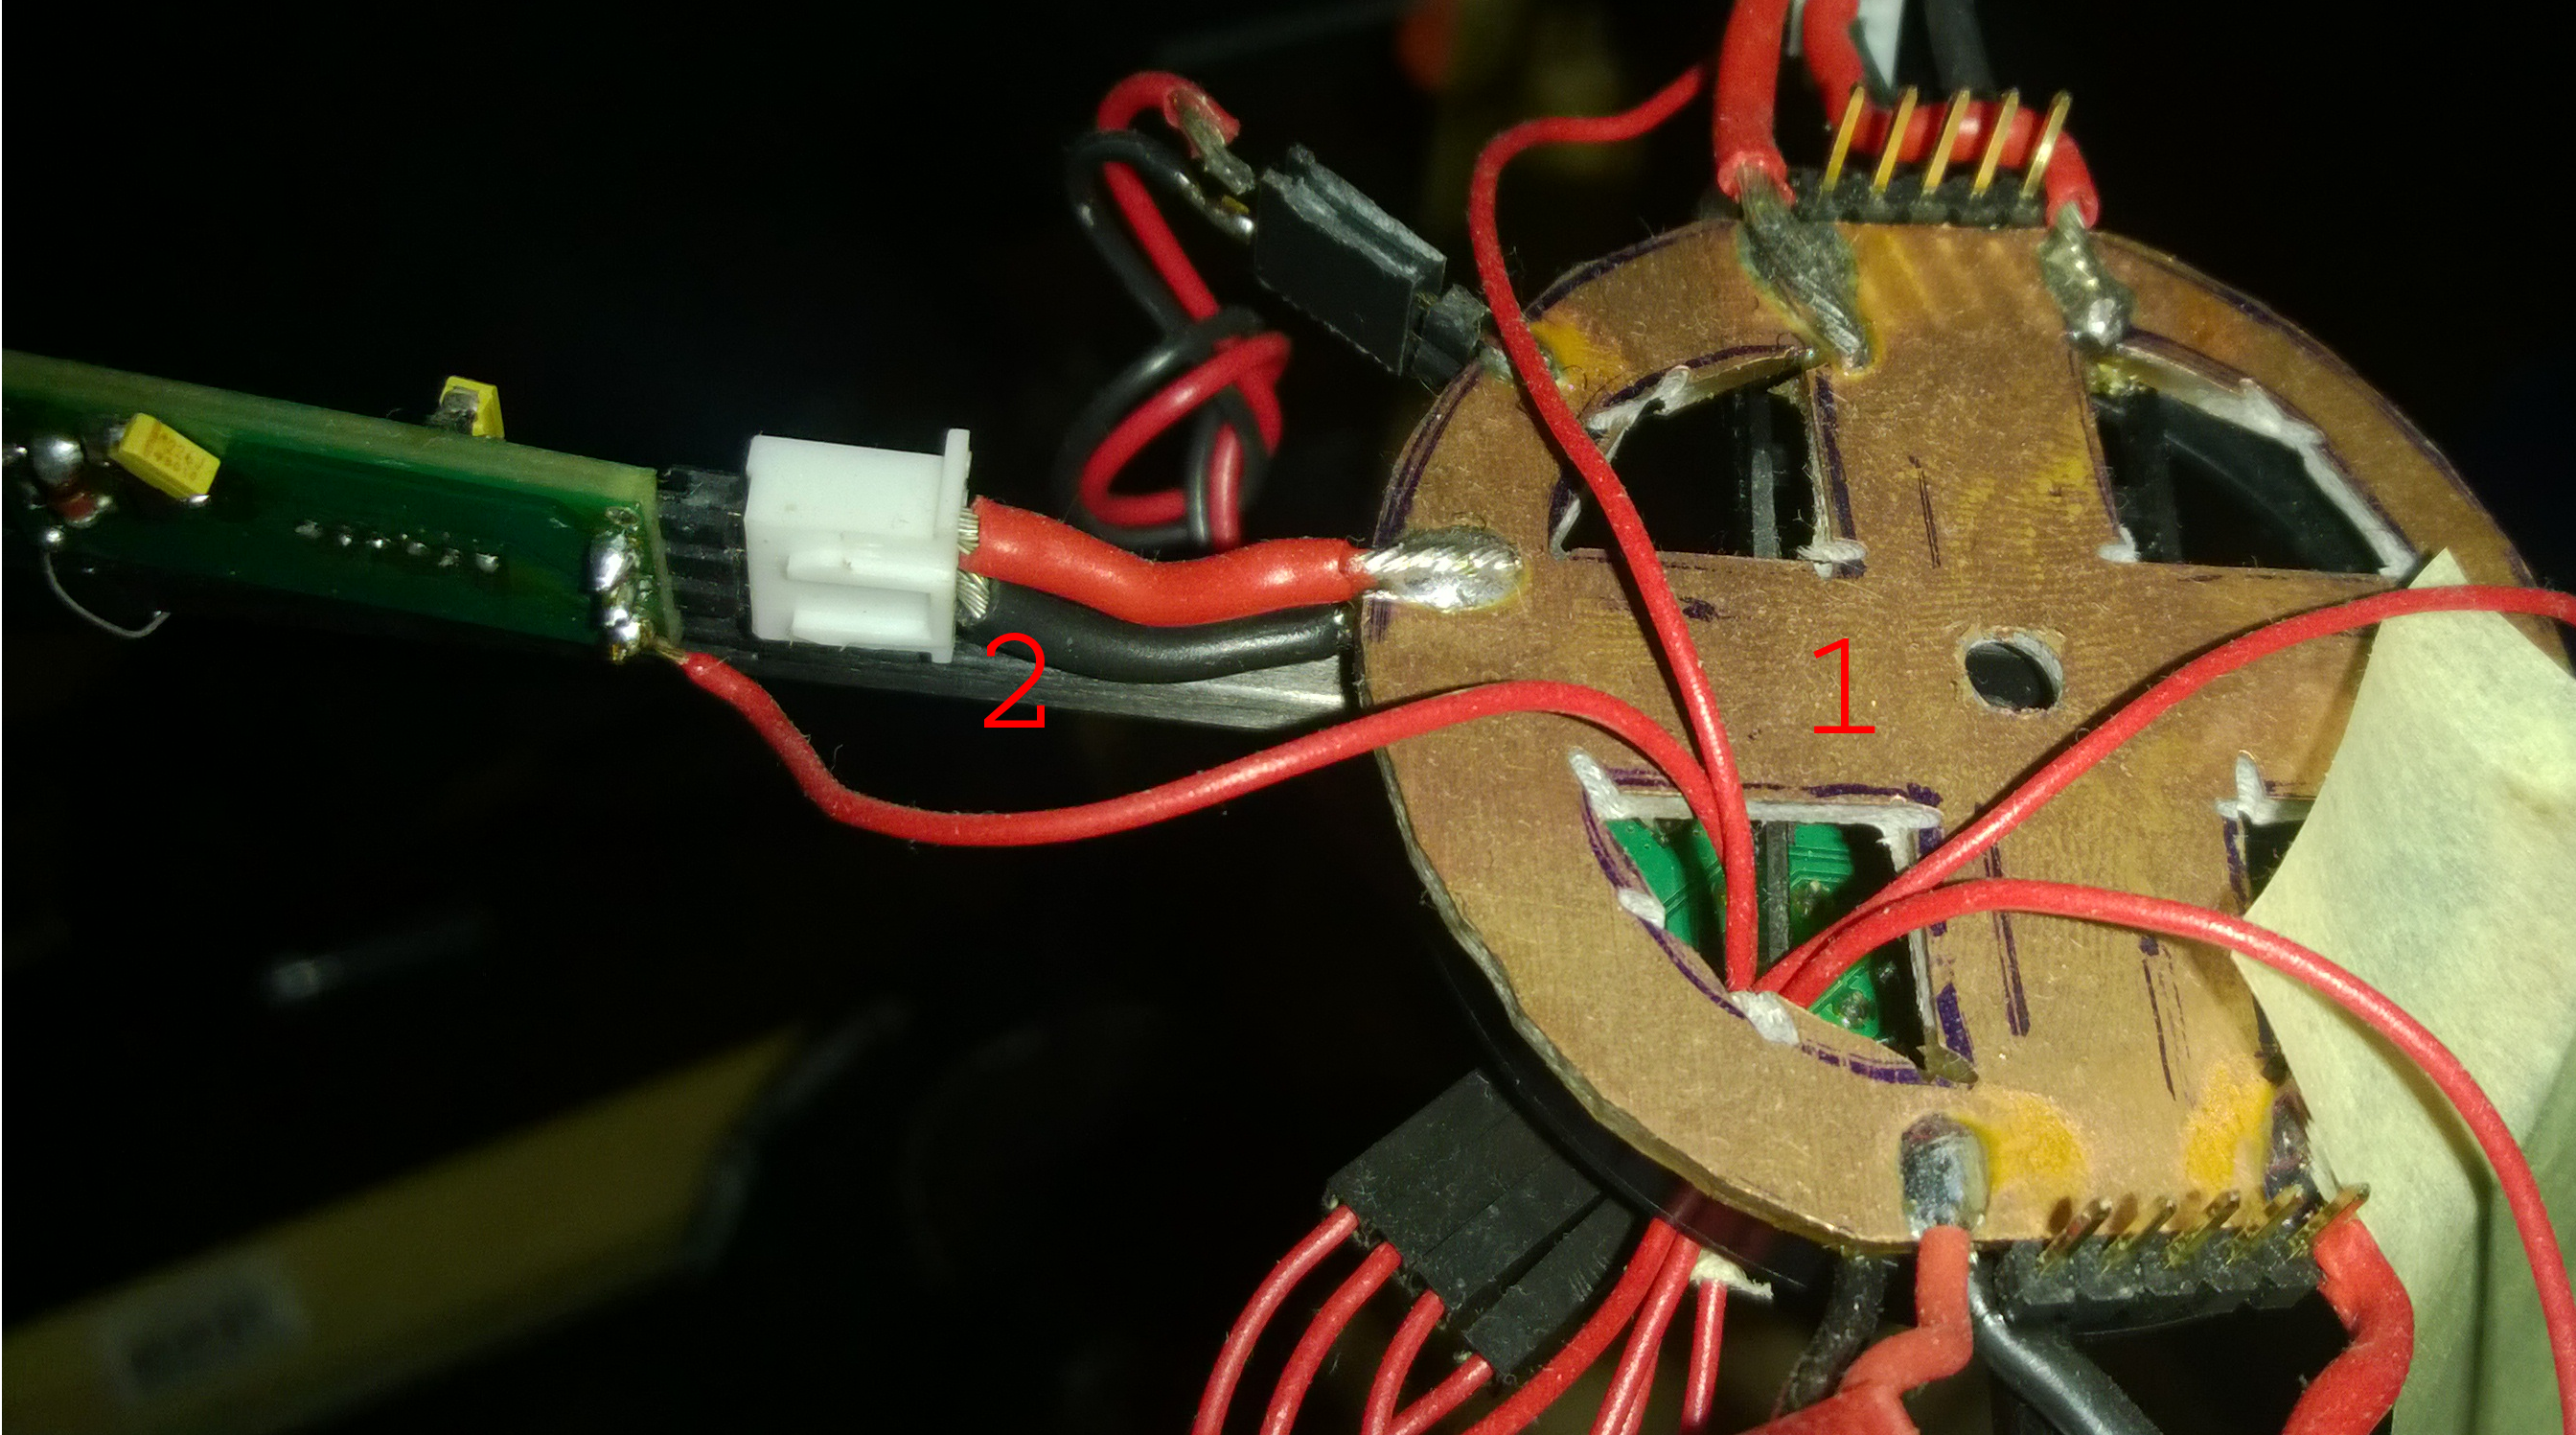
\includegraphics[scale=0.15]{Pictures/PowerDistributionBoard.png}
		%\rule{35em}{0.5pt}
	\caption[Zdjęcie płytki rozprowadzającej zasilanie w kwadrokopterze (1) oraz skróconych i pogrubionych przewodów zasilających sterownik silnika (2)]{Zdjęcie płytki rozprowawdzającej zasilanie w kwadrokopterze (1) oraz skróconych i pogrubionych przewodów zasilających sterownik silnika (2)}
	\label{fig:PowerDistribudionBoard}
\end{figure}

Rysunek ~\ref{fig:PowerDistribudionBoard} przedstawia płytkę rozprowadzającą zasilanie w kwadrokopterze opracowaną na podstawie wyników testów wszystkich czterech kontrolerów silników. Wykonano ją z dwustronnego laminatu, wykorzystując górną stronę płytki na rozprowadzenie masy akumulatora zasilającego kwadrokopter, a dolną stronę na podłączenie jego dodatniego bieguna zasilania. Po zamontowaniu płytki w kwadrokopterze problemy wynikające ze spadków napięcia na przewodach zasilających sterowniki silników przestały występować. W dalszym przebiegu testów regulacja pracy silników przebiegała bez problemów.

\section{Testy kontrolera lotu kwadrokoptera}

\begin{figure}[H]
	\centering
	\includegraphics[scale=0.2]{Pictures/QuadrotorController_test.png}
		%\rule{35em}{0.5pt}
	\caption[Schemat blokowy zestawu testowego kontrolera lotu kwadrokoptera]{Schemat blokowy zestawu testowego kontrolera lotu kwadrokoptera}
	\label{fig:QuadrotorController_test}
\end{figure}

Rysunek ~\ref{fig:QuadrotorController_test} przedstawia schemat blokowy zestawu testowego użytego podczas testów kwadrokoptera. Komputer PC użytkownika wyposażony w moduł Bluetooth odpowiedzialny był za generowanie sygnałów testowych odbieranych i przetwarzanych po stronie testowanego układu. Testy kontrolera zostały podzielone na dwa etapy:
\begin{itemize}
	\item \textbf{Testy generowania sygnałów PWM} - testy te polegały na wysyłaniu testowych danych, które bez udziału jakiegokolwiek algorytmu kontroli przekładały się na współczynniki wypełnienia impulsów sterujących kontrolerami silników. Dane były przesyłane w postaci binarnej zgodnie z protokołem omówionym w poprzednim rozdziale, a reakcja kontrolera obserwowana była za pomocą oscyloskopu. Testy te miały przede wszystkim sprawdzić działanie komunikacji radiowej, stabilność implementacji odbioru danych po stronie kontrolera lotu oraz prawidłowość generowanych sygnałów sterujących kontrolerami silników.
	\item \textbf{Testy komunikacji z czujnikiem MPU-6050} - testy te polegały na odczytywaniu wartości pomiarów z akcelerometru i żyroskopu oraz wysyłaniu ich w postaci tekstowej do komputera PC, gdzie następowała weryfikacja ich poprawności. W ich trakcje dokonywano zmiany położenia kątowego modułu czujników w przestrzeni weryfikując jednocześnie zmiany wartości odebranych pomiarów.  
	\item \textbf{Wstępne testy algorytmu stabilizacji i kontroli lotu} - testy te polegały na wysyłaniu binarnych wartości zadanego ciągu silników oraz prędkości kątowych kwadrokoptera wokół trzech osi układu współrzędnych, a następnie na obserwacji generowanych sygnałów sterujących. Ich celem było sprawdzenie stabilności algorytmu kontroli lotu kwadrokoptera oraz przetestowanie implementacji regulatorów PID.   
\end{itemize}


\section{Testy aplikacji użytkownika}

Krokiem, który następował po testach prototypów kontrolerów silników oraz kontrolera lotu, były testy aplikacji użytkownika do strojenia parametrów lotu oraz do kontroli kwadrokoptera. Obie te aplikacje pomimo zapewniania użytkownikowi zupełnie innych funkcji przy komunikacji z kwadrokopterem w gruncie rzeczy realizują to samo zadanie, polegające na przetwarzaniu poleceń wydawanych za pomoca interfejsu graficznego na odpowiednie komendy wysyłane do kontrolera lotu. 

\begin{figure}[H]
	\centering
	\includegraphics[scale=0.2]{Pictures/TestyAplikacji.png}
		%\rule{35em}{0.5pt}
	\caption[Schemat blokowy zestawu testowego aplikacji użytkownika]{Schemat blokowy zestawu testowego aplikacji użytkownika}
	\label{fig:UserAplication_test}
\end{figure}

Rysunek ~\ref{fig:UserAplication_test} przedstawia zestaw testowy, którego użyto do testów obu aplikacji użytkownika wspomnianych we wcześniejszej części tego podrozdziału. Aplikacja wysyłała odpowiednie komendy, w zależności od akcji podjętych przez użytkownika, przez interfejs Bluetooth. Dane te trafiały następnie do modułu HC-06 który wysyłał je przez interfejs UART do konwertera UART-USB widzianego przez komputer PC jako port szeregowy. W omawianym zestawie testowym nie użyto modułu Bluetooth wbudowanego w komputer PC, lecz zewnętrznego modułu identycznego do tego, który został zamontowany w kwadrokopterze, w celu odtworzenia docelowych warunków komunikacji radiowej. 

Testy aplikacji użytkownika miały na celu zbadanie stabilności jej działania, oraz sprawdzenie poprawności generowanych komend. Dane odbierane po stronie komputera PC wyświetlane były w postaci binarnej i analizowane pod kątem zgodności z definicją protokołu komunikacyjnego oraz logicznej spójności danych.

\section{Strojenie regulatorów PID kwadrokoptera}

Ostatnim etapem uruchomienia kwadrokoptera było nastrojenie jego regulatorów PID. Aby urządzenie miało zapewnioną stabilizację w płaszczyźnie poziomej, nalezy odpowiednio nastroić regulatory odpowiedzialne za utrzymanie zadanej prędkości kątowej wokół osi X oraz Y. Dokonuje się tego przez unieruchomienie dowolnej pary przeciwległych silników oraz zawieszenie kwadrokoptera na odpowiadającej im pozostałej parze ramion tak, aby mógł obracać się wokół osi kalibrowanego regulatora.

\begin{figure}[H]
	\centering
	\includegraphics[scale=0.15]{Pictures/QuadroTestStation.jpg}
		%\rule{35em}{0.5pt}
	\caption[Stanowisko testowe służące do strojenia regulatorów PID kwadrokoptera]{Stanowisko testowe służące do strojenia regulatorów PID kwadrokoptera}
	\label{fig:QuadroTestStation}
\end{figure}

Rysunek ~\ref{fig:QuadroTestStation} przedstawia stanowisko użyte do strojenia regulatorów PID dla osi X oraz Y kwadrokoptera. Składa się ono z podstawy, do której przymocowano dwie pionowe metalowe rury. Na ich końcach przymocowano poziomy aluminiowy pręt, do którego za pomocą specjalnie zaprojektowanych łączników przymocowany został kwadrokopter. Stanowisko zostało zaprojektowane w taki sposób, aby mogło zostać wykonane możliwie niskim kosztem, z łatwo dostępnych materiałów.  

\begin{figure}[H]
	\centering
	\includegraphics[scale=0.12]{Pictures/QuadroTestStationZoom.jpg}
		%\rule{35em}{0.5pt}
	\caption[System mocowania kwadrokoptera do stanowiska testowego]{System mocowania kwadrokoptera do stanowiska testowego}
	\label{fig:QuadroTestStationZoom}
\end{figure}

Rysunek ~\ref{fig:QuadroTestStationZoom} przedstawia zbliżenie kwadrokoptera ukazujące dokładnie sposób jego mocowania do stanowiska testowego. Widoczna na zdjęciu wersja łączników musiała zostać poprawiona w związku z faktem, iż ich konstrukcja wymuszała znaczne odsunięcie środka ciężkości kwadrokoptera od jego osi obrotu, przez co pojawiały się błędy w trakcie testowania algorytmu kontroli lotu. 

\begin{figure}[H]
	\centering
	\includegraphics[scale=0.12]{Pictures/QuadroTestStationZoom.jpg}
		%\rule{35em}{0.5pt}
	\caption[System mocowania kwadrokoptera do stanowiska testowego]{System mocowania kwadrokoptera do stanowiska testowego}
	\label{fig:QuadroTestStationZoom2}
\end{figure}

Rysunek ~\ref{fig:QuadroTestStationZoom2} przedstawia poprawioną wersję montażu kwadrokoptera do stanowiska testowego. Jak widać kształt łączników został tak zmieniony, aby oś obrotu pokrywała się w dużej mierze z położeniem środka ciężkości kwadrokoptera. Co więcej, nowe łączniki umożliwiają zmianę położenia osi obrotu względem ramy kwadrokoptera, dzięki czemu potencjalne zmiany jego środka ciężkości nie będą stwarzać problemów w trakcie testów. Drugą widoczną zmianą jest rozcięcie aluminiowego pręta na dwie części, co było koniecznością, jako że przy zamontowaniu nowych łączników zahaczałby on o ramę kwadrokoptera. 
 
% Chapter Template

\chapter{Wnioski} % Main chapter title

\label{Chapter8} % Change X to a consecutive number; for referencing this chapter elsewhere, use \ref{ChapterX}

\lhead{Rozdział 8. \emph{Wnioski}} % Change X to a consecutive number; this is for the header on each page - perhaps a shortened title

Celem niniejszej pracy było zapoznanie się z zasadą działania i stabilizacją lotu czterowirnikowych śmigłowców. Jako że autor pracy w chwili rozpoczęcia realizacji projektu nie posiadał żadnego doświadczenia w tworzeniu zdalnie sterowanych robotów, nacisk położono na prostotę projektowanych rozwiązań. Docelowo starano się osiągnąć prostą i~uniwersalną konstrukcję, stanowiącą punkt wyjściowy dla przyszłych wersji kwadrokoptera.

W ramach pracy wykonano następujące zadania:
\begin{itemize}
	\item Opracowano projekt kwadrokoptera:
	\begin{itemize}
		\item Opracowano modułową koncepcję urządzenia z podziałem na kontroler lotu i sterowniki silników
		\item Określono liczbę procesorów oraz określono zadania, za które są odpowiedzialne
		\item Stworzono schematy elektryczne oraz projekty płytek drukowanych dla układów kontrolera lotu i sterowników silników
		\item Dokonano montażu prototypu
		\item Wykorzystując dostępne biblioteki programowe, napisano algorytm stabilizacji i kontroli lotu kwadrokoptera
		\item Opracowano binarny protokół używany do komunikacji z kwadrokopterem
	\end{itemize}
	\item Napisano aplikacje uzytkownika:
	\begin{itemize}
		\item Aplikacja przeznaczona na platformę Android, służąca do kontroli kwadrokoptera
		\item Aplikacja przeznaczona na platformę PC, służąca do testów oprogramowania kwadrokoptera oraz strojenia parametrów algorytmu kontroli lotu
	\end{itemize}
	\item Opracowano stanowisko testowe, przeznaczone do strojenia algorytmu kwadrokoptera	
	\item Dokonano testów wszystkich zaprojektowanych modułów elektronicznych oraz aplikacji
	\item Dokonano strojenia algorytmu kwadrokoptera
\end{itemize}

Efektem wykonania zadań wymienionych powyżej jest opracowanie kwadrokoptera będącego uniwersalnym modułowym urządzeniem, które w prosty sposób może być modyfikowane i rozszerzane o nowe moduły elektroniczne (np. nowe moduły transmisji radiowej, dodatkowe moduły czujników). 
Zaprojektowane urządzenie spełnia wszystkie założenia projektowe i wymagania techniczne, co dowodzi słuszności zastosowanych rozwiązań.
W ramach projektu stworzono dwie wersje urządzenia. Błędy wykryte w pierwszej rewizji kwadrokoptera zostały poprawione w rewizji drugiej, która po przejściu testów układów elektronicznych oraz oprogramowania stała się finalną rewizją prezentowaną w pracy. 

 
%\chapter{BibTest}
\label{Chapter9}
\lhead{Chapter 9. \emph{BibTest}}

\cite{quadro1} 
\cite{quadro2} 
%\cite{quadro3} 
\cite{quadro4} 
\cite{quadro5} 
\cite{quadro6} 
\cite{quadro7} 
\cite{quadro8} 
\cite{quadro9} 
\cite{quadro10} 
\cite{quadro11} 
\cite{quadro12} 
\cite{quadro13} 
\cite{quadro14} 
\cite{quadro15} 
\cite{quadro16} 
\cite{quadro17} 
\cite{quadro18} 
\cite{quadro19} 
\cite{quadro20} 
\cite{quadro21} 
\cite{quadro22} 
\cite{quadro23} 
\cite{quadro24}

\cite{mems1}
\cite{mems2}
\cite{mems3}
\cite{mems4}

\cite{filters1}
\cite{filters2}
\cite{filters3}

\cite{ds_atmega328p}
\cite{ds_attiny85}
\cite{ds_mpu6050}
\cite{ds_mpu6050rm}
\cite{ds_avrpid}
\cite{ds_ardupilot}


%----------------------------------------------------------------------------------------
%	THESIS CONTENT - APPENDICES
%----------------------------------------------------------------------------------------

%\addtocontents{toc}{\vspace{2em}} % Add a gap in the Contents, for aesthetics

%\appendix % Cue to tell LaTeX that the following 'chapters' are Appendices

% Include the appendices of the thesis as separate files from the Appendices folder
% Uncomment the lines as you write the Appendices

%\input{Appendices/AppendixA}
%\input{Appendices/AppendixB}
%\input{Appendices/AppendixC}

\addtocontents{toc}{\vspace{1.5em}} % Add a gap in the Contents, for aesthetics

\backmatter

%----------------------------------------------------------------------------------------
%	BIBLIOGRAPHY
%----------------------------------------------------------------------------------------
%\setcounter{biburllcpenalty}{7000}
%\setcounter{biburlucpenalty}{8000}

\label{Bibliography}

\lhead{\emph{Bibliografia}} % Change the page header to say "Bibliography"

\bibliographystyle{unsrtnat} % Use the "unsrtnat" BibTeX style for formatting the Bibliography

\bibliography{Bibliography} % The references (bibliography) information are stored in the file named "Bibliography.bib"

\end{document}  
